% \documentclass[paper=a4, fontsize=11pt]{scrartcl} % A4 paper and 11pt font size
\documentclass[11pt, a4paper]{book}
\usepackage[a4paper, total={5.25in, 8.75in}]{geometry}
\usepackage[T1]{fontenc} % Use 8-bit encoding that has 256 glyphs
\usepackage[utf8]{inputenc}
\usepackage{fourier} % Use the Adobe Utopia font for the document - comment this line to return to the LaTeX default
\usepackage{listings} % para insertar código con formato similar al editor
\usepackage[spanish, es-tabla]{babel} % Selecciona el español para palabras introducidas automáticamente, p.ej. "septiembre" en la fecha y especifica que se use la palabra Tabla en vez de Cuadro
\usepackage{url} % ,href} %para incluir URLs e hipervínculos dentro del texto (aunque hay que instalar href)
\usepackage{graphics,graphicx, float} %para incluir imágenes y colocarlas
\usepackage[gen]{eurosym} %para incluir el símbolo del euro
\usepackage{cite} %para incluir citas del archivo <nombre>.bib
\usepackage{enumerate}
\usepackage{hyperref}
\usepackage{graphicx}
\usepackage{adjustbox}
\usepackage{booktabs}
\usepackage{dirtree}
\usepackage{float}
\usepackage{placeins}

\usepackage{tabularx}
\newcolumntype{L}{>{\raggedright\arraybackslash}X}
\newcolumntype{R}{>{\raggedleft\arraybackslash}X}

\usepackage[table,xcdraw]{xcolor}
\hypersetup{
	colorlinks=true,	% false: boxed links; true: colored links
	linkcolor=black,	% color of internal links
	urlcolor=cyan,		% color of external links
}

\renewcommand{\familydefault}{\sfdefault}
\usepackage{fancyhdr} % Custom headers and footers
\pagestyle{fancyplain} % Makes all pages in the document conform to the custom headers and footers
\fancyhead[L]{} % Empty left header
\fancyhead[C]{} % Empty center header
\fancyhead[R]{Ángel Gómez Martín} % My name
\fancyfoot[L]{} % Empty left footer
\fancyfoot[C]{} % Empty center footer
\fancyfoot[R]{\thepage} % Page numbering for right footer
%\renewcommand{\headrulewidth}{0pt} % Remove header underlines
\renewcommand{\footrulewidth}{0pt} % Remove footer underlines
\setlength{\headheight}{13.6pt} % Customize the height of the header
\setlength{\parskip}{1ex}

\usepackage{titlesec, blindtext, color}
\definecolor{gray75}{gray}{0.75}
\newcommand{\hsp}{\hspace{20pt}}
\titleformat{\chapter}[hang]{\Huge\bfseries}{\thechapter\hsp\textcolor{gray75}{|}\hsp}{0pt}{\Huge\bfseries}
\setcounter{secnumdepth}{4}
\usepackage[Lenny]{fncychap}

\definecolor{gray97}{gray}{.97}
\definecolor{gray75}{gray}{.75}
\definecolor{gray45}{gray}{.45}
\definecolor{gray30}{gray}{.94}

\lstdefinestyle{tree}{
literate=
    {├}{{\smash{\raisebox{-1ex}{\rule{1pt}{\baselineskip}}}\raisebox{0.5ex}{\rule{1ex}{1pt}}}}1 
    {└}{{\smash{\raisebox{0.5ex}{\rule{1pt}{\dimexpr\baselineskip-1.5ex}}}\raisebox{0.5ex}{\rule{1ex}{1pt}}}}1 
    {─}{{\raisebox{0.5ex}{\rule{1.5ex}{1pt}}}}1 
    {│}{{\smash{\raisebox{-1ex}{\rule{1pt}{\baselineskip}}}\raisebox{0.5ex}{\rule{1ex}{0pt}}}}1 
}

\lstset{
	frame=Ltb,
    framerule=0.5pt,
    aboveskip=0.5cm,
    framextopmargin=3pt,
    framexbottommargin=3pt,
    framexleftmargin=0.1cm,
    framesep=0pt,
    rulesep=.4pt,
    backgroundcolor=\color{gray97},
    rulesepcolor=\color{black},
    stringstyle=\ttfamily,
    showstringspaces = false,
    basicstyle=\scriptsize\ttfamily,
    commentstyle=\color{gray45},
    keywordstyle=\bfseries,
    numbers=left,
    numbersep=6pt,
    numberstyle=\tiny,
    numberfirstline = false,
    breaklines=true,
}
 
\lstset{
     literate=%
         {á}{{\'a}}1
         {í}{{\'i}}1
         {é}{{\'e}}1
         {ý}{{\'y}}1
         {ú}{{\'u}}1
         {ó}{{\'o}}1
         {ě}{{\v{e}}}1
         {š}{{\v{s}}}1
         {č}{{\v{c}}}1
         {ř}{{\v{r}}}1
         {ž}{{\v{z}}}1
         {ď}{{\v{d}}}1
         {ť}{{\v{t}}}1
         {ň}{{\v{n}}}1                
         {ů}{{\r{u}}}1
         {Á}{{\'A}}1
         {Í}{{\'I}}1
         {É}{{\'E}}1
         {Ý}{{\'Y}}1
         {Ú}{{\'U}}1
         {Ó}{{\'O}}1
         {Ě}{{\v{E}}}1
         {Š}{{\v{S}}}1
         {Č}{{\v{C}}}1
         {Ř}{{\v{R}}}1
         {Ž}{{\v{Z}}}1
         {Ď}{{\v{D}}}1
         {Ť}{{\v{T}}}1
         {Ň}{{\v{N}}}1                
         {Ů}{{\r{U}}}1    
}

\begin{document}
	\begin{titlepage}
\newlength{\centeroffset}
\setlength{\centeroffset}{-0.5\oddsidemargin}
\addtolength{\centeroffset}{0.5\evensidemargin}
\thispagestyle{empty}

\noindent\hspace*{\centeroffset}\begin{minipage}{\textwidth}

\centering
\includegraphics[width=0.9\textwidth]{logos/logo_ugr.jpg}\\[1.4cm]

\textsc{ \Large TRABAJO FIN DE MÁSTER\\[0.2cm]}
\textsc{ GRADO EN INGENIERÍA INFORMÁTICA}\\[1cm]

{\Huge\bfseries Matroos \\}
\noindent\rule[-1ex]{\textwidth}{3pt}\\[3.5ex]
{\large\bfseries Creación, configuración y despliegue de bots en \textit{Discord} }
\end{minipage}

\vspace{2.5cm}
\noindent\hspace*{\centeroffset}
\begin{minipage}{\textwidth}
\centering

\textbf{Autor}\\ {Ángel Gómez Martín}\\[2.5ex]
\textbf{Director}\\ {Juan Julián Merelo Guervós}\\[2cm]
\includegraphics[width=0.3\textwidth]{logos/etsiit_logo.png}\\[0.1cm]
\textsc{Escuela Técnica Superior de Ingenierías Informática y de Telecomunicación}\\
\textsc{---}\\
Granada, 7 de Julio de 2022
\end{minipage}
\end{titlepage}

	\thispagestyle{empty}

\begin{center}
{\large\bfseries Matroos \\ Creación, configuración y despliegue de bots en \textit{Discord}. }\\
\end{center}
\begin{center}
Ángel Gómez Martín\\
\end{center}

%\vspace{0.7cm}

\vspace{0.5cm}
\noindent{\textbf{Palabras clave}: software libre, \textit{Discord}, bot
\vspace{0.7cm}

\noindent{\textbf{Resumen}\\
	

\cleardoublepage

\begin{center}
{\large\bfseries Matroos \\ Creación, configuración y despliegue de bots en \textit{Discord}. }\\
\end{center}
\begin{center}
	Ángel Gómez Martín\\
\end{center}
\vspace{0.5cm}
\noindent{\textbf{Keywords}: \textit{open source}, \textit{Discord}, bot
\vspace{0.7cm}

\noindent{\textbf{Abstract}\\


\cleardoublepage

\thispagestyle{empty}

\noindent\rule[-1ex]{\textwidth}{2pt}\\[4.5ex]

D. \textbf{Juan Julián Merelo Guervós}, Profesor del Departamento de Arquitectura y Tecnología de Computadores de la Universidad de Granada.

\vspace{0.5cm}

\textbf{Informa:}

\vspace{0.5cm}

Que el presente trabajo, titulado \textit{\textbf{Matroos}},
ha sido realizado bajo mi supervisión por \textbf{Ángel Gómez Martín}, y autorizo la defensa de dicho trabajo ante el tribunal
que corresponda.

\vspace{0.5cm}

Y para que conste, expiden y firman el presente informe en Granada a Julio de 2022.

\vspace{1cm}

\textbf{El director: }

\vspace{5cm}

\noindent Fdo: Juan Julián Merelo Guervós



\chapter*{Agradecimientos}

A mi tutor, JJ, por ofrecerme su ayuda, conocimientos y acertados comentarios para la realización de este proyecto.

A mis padres, Elia y Ángel, por ser un pilar fundamental y por empujarme a seguir aprendiendo cosas nuevas y a superarme cada día.

A mi hermana Cristina, por apoyarme y echarme una mano siempre que lo he necesitado.

Y a Paula, por aguantarme más que nadie todo este tiempo.


	\newpage
	\tableofcontents

	\newpage
	\listoffigures

	\listoftables 
	\newpage

	\chapter{Introducción}

\textit{Discord}\cite{discord} es una aplicación de mensajería de uso tanto personal como en empresas. Es semejante a otras herramientas que se usan en ámbitos similares, como \textit{Slack}\cite{slack} o \textit{TeamSpeak}\cite{teamspeak}, y ofrece distintos servicios de comunicación, como mensajería instantánea, chat de voz e integración con bots y videojuegos.

Estos últimos elementos son bastante importantes, ya que la integración con videojuegos ha hecho que \textit{Discord} gane visibilidad en los últimos años; y la integración con bots ha hecho que la herramienta sea una herramienta mucho más interactiva que las otras mencionadas. Más información en el estado del arte.

En concreto, este proyecto se centra en los bots, que podrían definirse como herramientas que, haciendo uso de diferentes permisos, ayudan a automatizar tareas dentro de un servidor de \textit{Discord}. Las funciones de éstos son prácticamente ilimitadas, aunque las más populares son moderación de usuarios y mensajes, música, envío de contenido, noticias o encuestas.

Usuarios más avanzados (como por ejemplo, un administrador de sistemas, o alguien que controla distintos equipos) que quieren hacer uso de este software y de su sistema de bots se ven obligados a crear distintos bots muy específicos y en ocasiones poco reutilizables. Si bien se podrían programar comandos más específicos en un único bot, sería una tarea tediosa la reutilización entre diferentes ámbitos.

Incidiendo en el aspecto de la creación de bots forma más técnica, se observa que actualmente hay tres maneras de usar bots en \textit{Discord}:

\begin{itemize}
	\item \textbf{Usar bots ya existentes}. El bot ya se encuentra creado, configurado y desplegado, y solo es necesario agregarlo al servidor para poder disfrutar de sus funcionalidades.
	\item \textbf{Crear un bot a alto nivel}. Este caso es similar al anterior, ya que se trata de un bot genérico, que es configurable en cierta medida para cada servidor. Esta configuración se hace a través de algún tipo de herramienta (generalmente una aplicación web) que permite configurar los comandos deseados. Por otro lado, ya que están pensados para un público general, las posibilidades de configuración son escasas. Suelen tener algunas plantillas de comandos básicos, como temporizadores o respuestas automáticas.
	\item \textbf{Crear un bot a bajo nivel}. En este caso el bot se crea haciendo uso de las diferentes \textit{API} que ofrece \textit{Discord} para ello y la personalización es máxima. En cambio, es más tedioso, y requiere conocimientos extra que algunos usuarios pueden no tener (como programación). Además hay que tener en cuenta que el bot debe ser desplegado manualmente, por lo que requiere un esfuerzo extra.
\end{itemize}

Además, en el caso de que se quisieran desplegar distintos bots al mismo tiempo y administrarlos desde un mismo entorno, no sería posible, ya que cada uno de estos es una instancia distinta.

Por tanto, se pretende desarrollar un \textit{framework} para crear bots de \textit{Discord} configurables que sean capaces de conectar con diferentes sistemas. La principal motivación a la hora de desarrollar este sistema es encontrar la manera de centralizar la creación y la administración de bots de este tipo, además de resolver los diferentes problemas planteados:

\begin{itemize}
	\item Dificultad al crear bots con funcionalidades específicas.
	\item Poca configuración en aspectos más técnicos, como administración de sistemas.
	\item Dificultad de manejar el despliegue de distintos bots al mismo tiempo.
\end{itemize}

Es por tanto, un software pensado para usuarios mas avanzados, ya que los usuarios con menor conocimiento de las tareas administrativas sólo hacen uso de estos bots una vez ya desplegados a través de los servidores de \textit{Discord}.

	\chapter{Estado del arte}

En este capítulo se hace un repaso de las distintas soluciones que existen actualmente para la creación de bots de \textit{Discord} y la configuración de sus comandos.

\section{Contexto y definiciones previas}

Los bots actúan como un usuario más dentro de un servidor de \textit{Discord}. En cambio, debido a su naturaleza, deben ser agregados a los servidores por usuarios humanos. Se pueden crear infinidad de bots, por lo que han surgido páginas web (como \href{https://top.gg/}{top.gg} o \href{https://bots.ondiscord.xyz/}{Bots on Discord}) que permiten que los usuarios encuentren bots ya creados y desplegados listos para ser utilizados en sus servidores. Estos cuentan con funcionalidades específicas, por lo que no pueden modificarse por los usuarios.

Además de este tipo de bots y webs, han surgido otras plataformas que permiten que los usuarios creen y configuren sus propios bots. Estas son las que se desarrollan en este capítulo. A continuación se enumeran algunos conceptos que son interesantes conocer ya que se utilizan tanto en este capítulo como en el resto del documento.

Conceptos técnicos, que definen la manera en la que se estructuran, configuran y definen los bots:

\begin{itemize}
	\item \textbf{Comandos predefinidos}. Comandos cuya funcionalidad está ya definida (y por tanto programada) y no puede ser modificada por un usuario.
	\item \textbf{Comandos personalizados}. Comandos que se pueden crear a partir de comandos predefinidos que pueden utilizarse con distintos parámetros para modificar su comportamiento.
	\item \textbf{Comandos reutilizables}. Comandos personalizados que una vez configurados pueden utilizarse en distintos bots.
	\item \textbf{Despliegue de un bot}. Todas aquellas tareas y actividades que hacen que un bot se encuentre disponible para ser usado por usuarios.
	\item \textbf{Control del despliegue}. Capacidad de controlar y monitorizar el despliegue de bots en un sistema.
\end{itemize}

Conceptos relacionados con funcionalidades de \textit{Discord}:

\begin{itemize}
    \item \textbf{Comandos de moderación}. Comandos cuya funcionalidad se centra en la moderación de usuarios en los servidores de \textit{Discord}.
\end{itemize}

\section{Soluciones actuales}

Las soluciones actuales se podrían dividir en dos grupos, las herramientas \textit{no-code} y aquellas herramientas que hacen uso de programación. En ambas la interacción con el sistema se hace a través de una aplicación web y, además, suelen tener una apariencia muy similar, siendo las \textit{no-code} algo más complejas de usar. Las primeras se centran en usuarios con menor conocimiento técnico, abstrayendo todos los detalles de este tipo. En cambio, las segundas son utilizadas por aquellos usuarios con un conocimiento informático más amplio.

En las siguientes secciones se incluyen las herramientas con características más interesantes. Por otro lado, para cada herramienta se incluye una tabla como la siguiente, donde se resumen las características más importantes de cada una de ellas.

\FloatBarrier
\begin{table}[h]
    \centering
    \def\arraystretch{1.25}
    \begin{adjustbox}{max width=\textwidth}
    \begin{tabularx}{325px}{|l|L|}
    \hline
        \multicolumn{2}{|c|}{\textbf{Nombre de la herramienta}} \\ \hline
    \hline
        \textbf{Tipo de comandos} & El tipo de comandos que provee la herramienta, y la cantidad de comandos personalizados que se pueden crear. \\ \hline
        \textbf{Comandos reutilizables} & Si los comandos se pueden reutilizar entre bots o no. \\ \hline
        \textbf{Control del despliegue} & Si el usuario tiene control del despliegue del bot o no. \\ \hline
        \textbf{Número de bots} & La cantidad de bots que el usuario puede crear y configurar. \\ \hline
        \textbf{Experiencia} & La experiencia de usuario a la hora de utilizar las herramientas. \\ \hline
        \textbf{Personalización extra} & Si la herramienta permite una personalización más avanzada, y si es de pago o no. \\ \hline
        \textbf{Características} & Las funcionalidades configurables en los bots. \\ \hline
        \textbf{Logs} & Si permiten que los usuarios tengan acceso a los logs de los bots. \\ \hline
        \textbf{Premium} & Coste de los planes de pago de la herramienta. \\ \hline
    \end{tabularx}
    \end{adjustbox}
    \caption{Cuadro resumen de las características de una herramienta.}
\end{table}
\FloatBarrier

\subsection{Herramientas \textit{no-code}}

Estas herramientas permiten la creación de bots sin hacer uso de recursos de programación o similares. Cuentan con un repertorio de comandos predefinidos, de los cuales se pueden crear comandos personalizados modificando los parámetros de estos. Esto se hace a través de interfaces gráficas sencillas compuestas por formularios y otros elementos.

Por ejemplo, el comando predefinido más común sirve para enviar mensajes. A partir de este comando se pueden crear distintos comandos personalizados, cambiando la palabra clave que los usuarios deben introducir (en los canales de texto) para activar el comando y el mensaje que el bot debe enviar.

En general la mayoría tienen una serie de funcionalidades gratuitas, teniendo que suscribirse a un plan de pago mensual para obtener funcionalidades extra. Estas suscripciones suelen tener un coste aproximado de cinco dólares mensuales, pudiendo comprar suscripciones anuales o incluso de por vida y suelen ofrecer un repertorio de comandos más amplio, conexiones con redes sociales, estadísticas de uso e incluso \textit{logging}.

En la mayoría de casos estas plataformas cuentan con un único bot que se debe agregar al servidor de \textit{Discord} deseado. Esto implica que el uso de estos servicios no permite por tanto agregar varios bots con distintas funcionalidades a un mismo servidor. Si un usuario utiliza \textit{ProBot} (servicio que se explica en detalle a continuación), entonces el bot que proporciona \textit{ProBot} sólo podrá utilizarse una sola vez por servidor.

En ellas se puede observar también uno de los principales problemas ya mencionados, la muy reducida personalización y reutilización de los comandos. En estos sistemas no se puede crear un comando específico con una funcionalidad concreta, sino que se basan en funcionalidades predefinidas no reutilizables.

Estas funcionalidades predefinidas son en su mayoría de moderación de usuarios y envío de mensajes, y no se pueden reutilizar entre distintos bots. Además, debido a la estructura y arquitectura de estas plataformas, los usuarios no pueden ampliar el repertorio de comandos, teniendo que conformarse con los existentes.

\subsubsection{\textit{ProBot}}

\href{https://probot.io/}{\textit{ProBot}} es sin duda la más interesante de las herramientas \textit{no-code} debido a que permite crear ilimitados comandos personalizados, siendo la principal desventaja que estos comandos son predefinidos, y no se puede cambiar su funcionalidad. Los comandos predefinidos se centran en moderación y mensajes automáticos, por lo que las posibilidades no son muy amplias.

A favor de esta herramienta también destaca que es sencilla de utilizar, la interfaz web intenta imitar a la de \textit{Discord} y es intuitiva. Por contra, es bastante intrusiva la modalidad \textit{premium}, ya que muchas secciones sugieren la compra de esta modalidad. Además es imposible controlar el despliegue del bot, y no es posible reutilizar comandos.

Sus características son:

\FloatBarrier
\begin{table}[h]
    \centering
    \def\arraystretch{1.25}
    \begin{adjustbox}{max width=\textwidth}
    \begin{tabularx}{325px}{|l|L|}
    \hline
        \multicolumn{2}{|c|}{\textbf{\textit{ProBot}}} \\ \hline
    \hline
        \textbf{Tipo de comandos} & Predefinidos (ilimitados) \\ \hline
        \textbf{Comandos reutilizables} & No \\ \hline
        \textbf{Control del despliegue} & No \\ \hline
        \textbf{Número de bots} & 1, único \\ \hline
        \textbf{Experiencia} & Sencilla \\ \hline
        \textbf{Personalización extra} & Requiere \textit{premium} (mensualidades) \\ \hline
        \textbf{Características} & Moderación, estadísticas, mensajes automáticos, música \\ \hline
        \textbf{Logs} & No \\ \hline
        \textbf{Premium} & \$60 al año \\ \hline
    \end{tabularx}
    \end{adjustbox}
    \caption{Características de \textit{ProBot}.}
\end{table}
\FloatBarrier

\FloatBarrier
\begin{figure}[h]
	\centering
	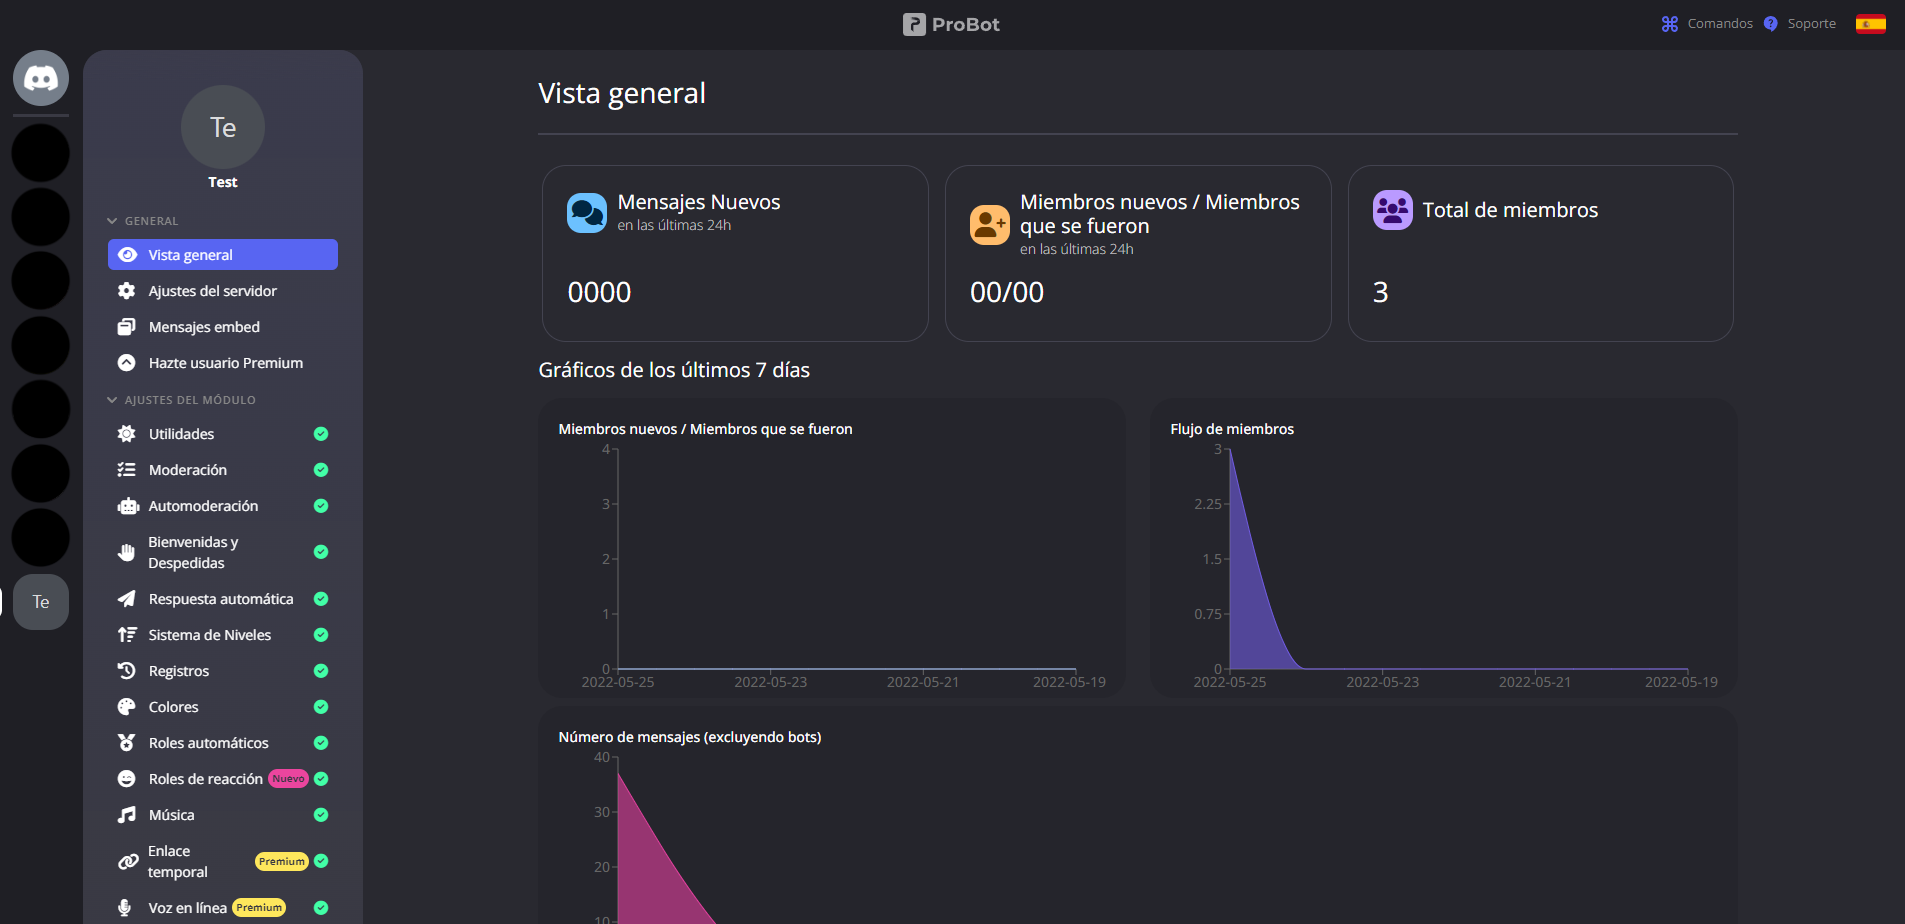
\includegraphics[width=1\textwidth]{img/probot.png}
	\caption{Interfaz web de \textit{ProBot}.}
\end{figure}
\FloatBarrier

\subsubsection{\textit{Mee6}}

\href{https://mee6.xyz/}{\textit{Mee6}} es otra herramienta muy similar a la anterior, siendo la principal diferencia que en este caso los comandos personalizados se limitan a 5. Por contra, tiene un mayor catálogo de funcionalidades.

De nuevo no es posible controlar el despliegue del bot, como tampoco es posible crear otro bot y agregarlo a un mismo servidor, o reutilizar comandos.

Sus características son:

\FloatBarrier
\begin{table}[h]
    \centering
    \def\arraystretch{1.25}
    \begin{adjustbox}{max width=\textwidth}
    \begin{tabularx}{325px}{|l|L|}
    \hline
        \multicolumn{2}{|c|}{\textbf{\textit{Mee6}}} \\ \hline
    \hline
        \textbf{Tipo de comandos} & Predefinidos (muy limitados, 5) \\ \hline
        \textbf{Comandos reutilizables} & No \\ \hline
        \textbf{Control del despliegue} & No \\ \hline
        \textbf{Número de bots} & 1, único \\ \hline
        \textbf{Experiencia} & Sencilla \\ \hline
        \textbf{Personalización extra} & Requiere \textit{premium} (mensualidades) \\ \hline
        \textbf{Características} & · Moderación, estadísticas, mensajes automáticos, música, temporizadores, \textit{quiz} / \textit{trivia} \\ \hline
        \textbf{Logs} & No \\ \hline
        \textbf{Premium} & \$50 al año / \$90 de por vida  \\ \hline
    \end{tabularx}
    \end{adjustbox}
    \caption{Características de \textit{Mee6}.}
\end{table}
\FloatBarrier

\FloatBarrier
\begin{figure}[h]
	\centering
	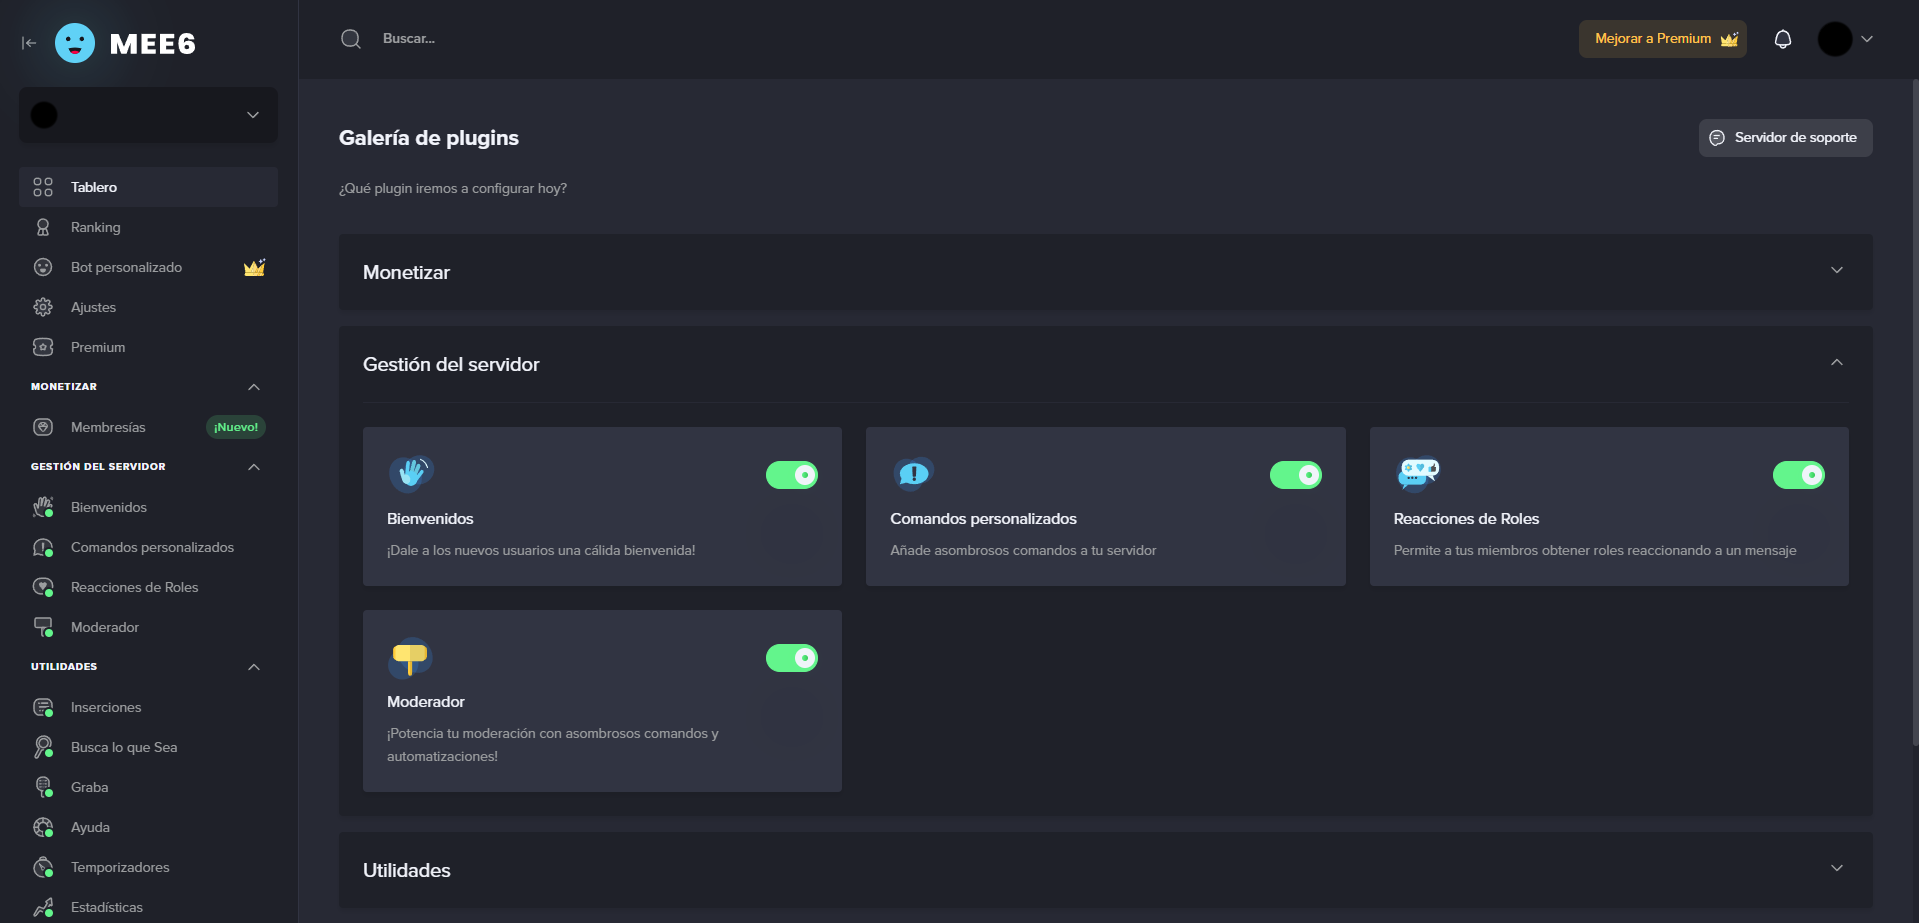
\includegraphics[width=1\textwidth]{img/mee6.png}
	\caption{Interfaz web de \textit{Mee6}.}
\end{figure}
\FloatBarrier


\subsubsection{\textit{BotGhost}}

\href{https://botghost.com/}{\textit{BotGhost}} es un híbrido entre \textit{ProBot} y \textit{Mee6}, ya que tiene características comunes de ambos. La principal característica de esta herramienta es que permite crear comandos personalizados haciendo uso de una serie de módulos que se pueden interconectar para definir el ciclo de vida de un comando.

Esta característica es muy interesante, pero está muy limitada y las funcionalidades que permite realizar se resumen en envío de mensajes y tareas de moderación de usuarios muy básicas. El plan \textit{premium} sería necesario en este caso para poder sacarle partido a esta funcionalidad.

Otro aspecto interesante es que se pueden crear distintos bots, hasta 50 distintos si se opta por la opción \textit{premium}. Sus características son las siguientes.

\FloatBarrier
\begin{table}[h]
    \centering
    \def\arraystretch{1.25}
    \begin{adjustbox}{max width=\textwidth}
    \begin{tabularx}{325px}{|l|L|}
    \hline
        \multicolumn{2}{|c|}{\textbf{\textit{BotGhost}}} \\ \hline
    \hline
        \textbf{Tipo de comandos} & Predefinidos (muy limitados, 5) \\ \hline
        \textbf{Comandos reutilizables} & Sí \\ \hline
        \textbf{Control del despliegue} & No (Sólo encendido y apagado) \\ \hline
        \textbf{Número de bots} & 1, único (50 con \textit{premium}) \\ \hline
        \textbf{Experiencia} & Compleja \\ \hline
        \textbf{Personalización extra} & Requiere \textit{premium} (mensualidades) \\ \hline
        \textbf{Características} & · Moderación, estadísticas, mensajes automáticos, temporizadores, integración con videojuegos, meteorología, música, \textit{quiz} / \textit{trivia} \\ \hline
        \textbf{Logs} & No \\ \hline
        \textbf{Premium} & \$60 al año / \$100 de por vida \\ \hline
    \end{tabularx}
    \end{adjustbox}
    \caption{Características de \textit{BotGhost}.}
\end{table}
\FloatBarrier

\FloatBarrier
\begin{figure}[h]
	\centering
	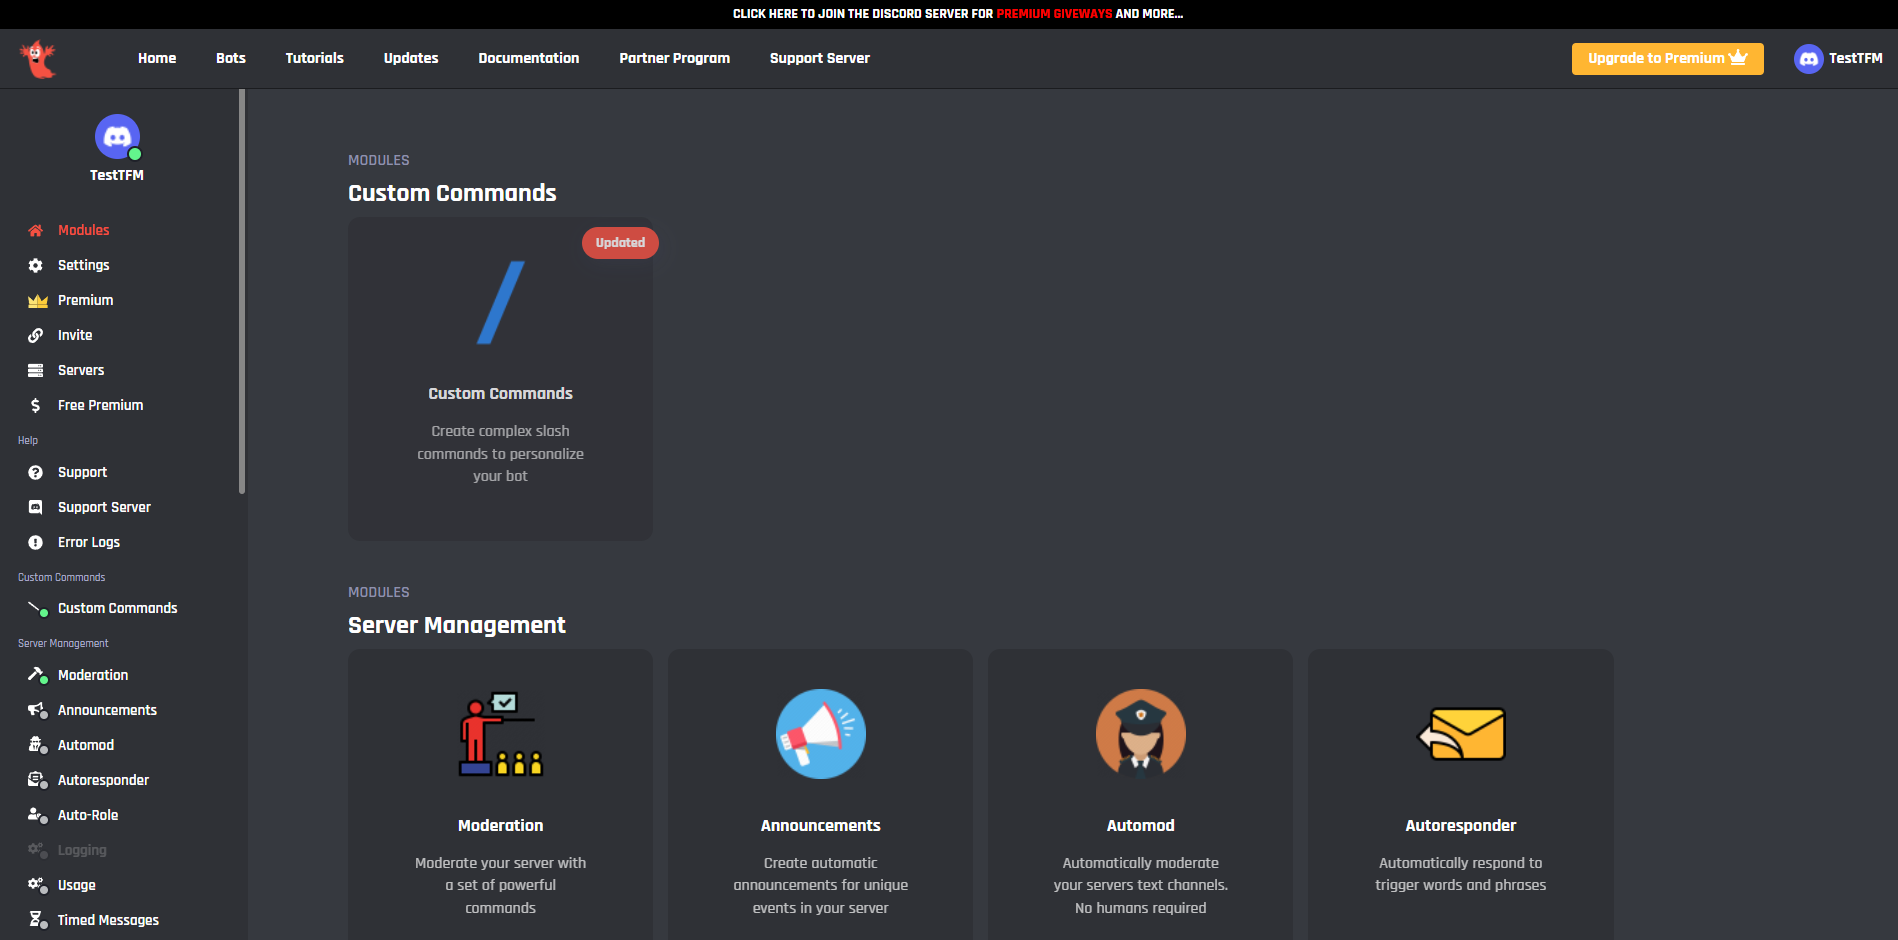
\includegraphics[width=1\textwidth]{img/botghost.png}
	\caption{Interfaz web de \textit{BotGhost}.}
\end{figure}
\FloatBarrier

\subsection{Herramientas de programación}

Actualmente existen multitud de librerías para distintos lenguajes de programación que permiten interactuar con la \textit{API} de \textit{Discord} y por tanto crear un bot. Así mismo existen herramientas híbridas que permiten esta creación de una manera más sencilla.

\subsubsection{\textit{Autocode}}

\href{https://autocode.com/}{\textit{Autocode}} es sin duda la herramienta mas interesante que existe de esta modalidad híbrida. Realmente es una plataforma que facilita la creación y despliegue de aplicaciones y servicios web, bots, y tareas de automatización permitiendo que los usuarios escriban sólo una parte del código (\textit{JavaScript}) de estos. Esta plataforma provee al usuario con un editor de código sencillo y de un explorador de archivos, recursos con los cuales puede crear el código.

De este modo el usuario sólo tiene que preocuparse por el código de la aplicación (o bot en este caso) que quiere crear, ya que del despliegue se encarga \textit{Autocode}. En su plan gratuito se pueden crear hasta 50 aplicaciones distintas, y permite la integración entre si de los distintos recursos que el usuario crea en la plataforma.

Sus características son:

\FloatBarrier
\begin{table}[h]
    \centering
    \def\arraystretch{1.25}
    \begin{adjustbox}{max width=\textwidth}
    \begin{tabularx}{325px}{|l|L|}
    \hline
        \multicolumn{2}{|c|}{\textbf{\textit{Autocode}}} \\ \hline
    \hline
        \textbf{Tipo de comandos} & Predefinidos + \textit{JS} \\ \hline
        \textbf{Comandos reutilizables} & No \\ \hline
        \textbf{Control del despliegue} & Sí (limitado) \\ \hline
        \textbf{Número de bots} & 50 gratis \\ \hline
        \textbf{Experiencia} & Algo complejo \\ \hline
        \textbf{Personalización extra} & Requiere \textit{premium} (mensualidades) \\ \hline
        \textbf{Especialidad} & Despliegue general de aplicaciones \\ \hline
        \textbf{Logs} & Sí (1-30 días) \\ \hline
        \textbf{Premium} & \$180 / \$1620 al año \\ \hline
    \end{tabularx}
    \end{adjustbox}
    \caption{Resumen de soluciones actuales.}
\end{table}
\FloatBarrier

\FloatBarrier
\begin{figure}[h]
	\centering
	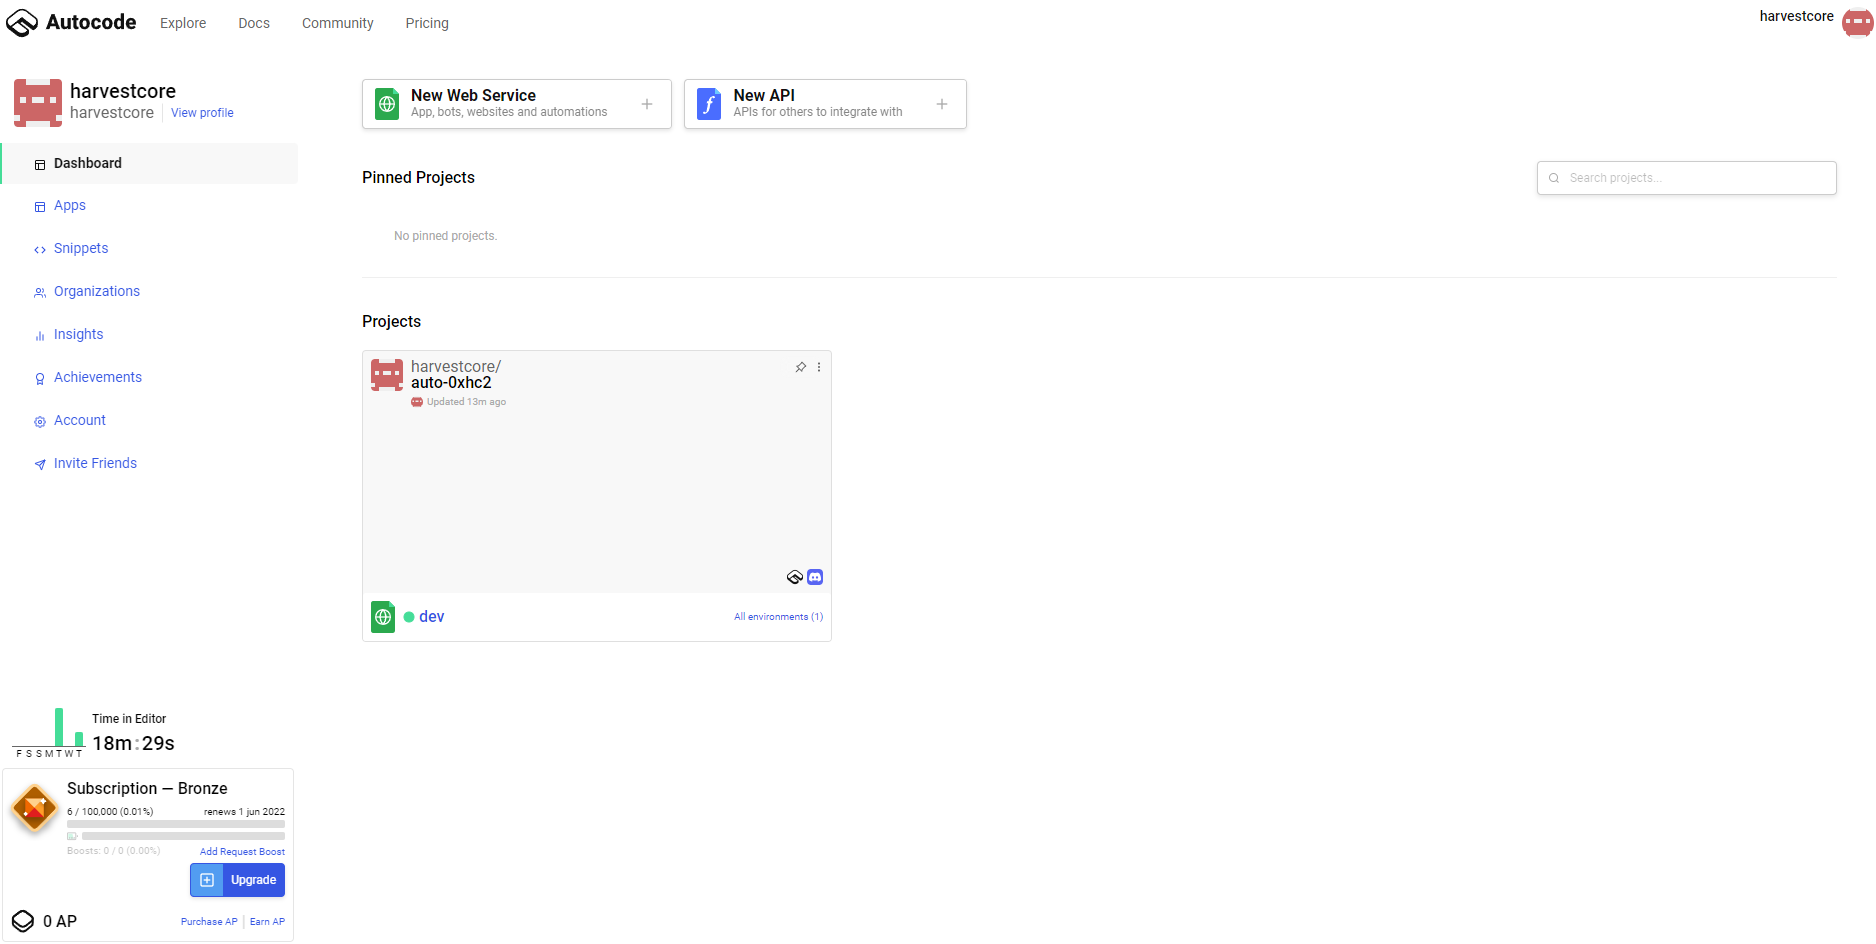
\includegraphics[width=1\textwidth]{img/autocode.png}
	\caption{Interfaz web de \textit{Autocode}.}
\end{figure}
\FloatBarrier

\subsubsection{Librerías de programación}

Las librerías de programación dan libertad total a la hora de crear un bot de \textit{Discord}, lo cual puede ser ideal en algunos casos. Las ventajas son obvias, ya que se puede crear cualquier tipo de comando y la reutilización es sencilla, pero en cambio, la gestión del despliegue puede ser compleja.

Por lo general todas las librerías permiten realizar casi las mismas funcionalidades, diferenciándose en aspectos como el rendimiento, la comunidad que las soporta o la facilidad de uso.

Algunos ejemplos de librerías son:

\begin{itemize}
	\item \textbf{\textit{C\#}}: \href{https://discordnet.dev/}{\textit{Discord.NET}}, \href{https://github.com/DSharpPlus/DSharpPlus}{\textit{DSharpPlus}}
	\item \textbf{\textit{Java}}: \href{https://github.com/DV8FromTheWorld/JDA}{\textit{JDA}}, \href{https://discord4j.com/}{\textit{Discord4J}}
	\item \textbf{\textit{C++}}: \href{https://dpp.dev/}{\textit{D++}}
	\item \textbf{\textit{JavaScript}}: \href{https://discord.js.org/}{\textit{discord.js}}
	\item \textbf{\textit{Golang}}: \href{https://github.com/bwmarrin/discordgo}{\textit{DiscordGo}}
	\item \textbf{\textit{Ruby}}: \href{https://github.com/shardlab/discordrb}{\textit{discordrb}}
\end{itemize}


\subsection{Comparativa de tiempos}

En esta sección se hace una comparativa del tiempo medio de desarrollo desde cero de un bot de \textit{Discord} usando las herramientas anterior mencionadas. Además se incluye tiempos de desarrollo usando tres lenguajes de programación: \textit{C\#}, \textit{JavaScript} y \textit{Python}.

Las mediciones incluyen todos los pasos necesarios para crear uno de estos bots con dos comandos personalizados. En el caso de las herramientas de programación se incluye desde la creación del proyecto hasta el despliegue (en local) de este.

Los dos comandos personalizados se han elegido al ser comunes en todas las plataformas mencionadas, además de sencillos de implementar. Son los siguientes:

\begin{itemize}
	\item Envío de un mensaje.
	\item Envío de un mensaje recurrente (cada cierto tiempo).
\end{itemize}

\FloatBarrier
\begin{table}[h]
    \centering
    \def\arraystretch{1.25}
    \begin{adjustbox}{max width=\textwidth}
    \begin{tabularx}{200px}{|l|R|}
    \hline
        \textbf{Herramienta} & \textbf{Tiempo (en minutos)} \\ \hline
    \hline
        ProBot & 5 \\ \hline
        Mee6 & 5 \\ \hline
        BotGhost & 10 \\ \hline
    \hline
        Autocode (JS) & 45 \\ \hline
    \hline
        JS & 85 \\ \hline
        C\# & 100 \\ \hline
        Python & 80 \\ \hline
    \end{tabularx}
    \end{adjustbox}
    \caption{Comparativa de tiempos de las distintas herramientas analizadas.}
\end{table}
\FloatBarrier

\section{Discusión}

Como se puede observar existen multitud de posibilidades a la hora de crear un bot de \textit{Discord}, y, aunque cumplen lo que prometen, se centran en aspectos muy concretos dejando otros bastante desatendidos.

En las herramientas \textit{no-code} los bots se centran principalmente en tareas de moderación, envío de mensajes, estadísticas e integración con videojuegos y redes sociales. Además, para sacarles partido es necesario el uso de los paquetes \textit{premium}, dejando de lado en el plan gratuito detalles específicos (y que serían ideales) como:

\begin{itemize}
	\item Reutilización de comandos.
	\item Creación de comandos con funcionalidad específica.
	\item Control del despliegue de los bots.
	\item Creación de distintos bots con distintas funcionalidades en un mismo sistema.
\end{itemize}

En el caso de las librerías de programación, aunque todas permiten el acceso a la \textit{API} de \textit{Discord}, cada una de ellas tiene una estructura distinta y los procedimientos para crear un bot o comandos son más o menos complejos. Si un usuario decidiese utilizarlas tendría flexibilidad completa a la hora de crear una estructura concreta, pero entonces tendría que dedicar en ese caso un tiempo necesario para diseñar algo funcional.

\textit{Autocode} es una buena alternativa a las soluciones anteriores, ya que se evita el tener que gestionar el despliegue de los bots y se eliminan algunas trabas de gestión del código, pero al igual que el uso de librerías toda la lógica recae en el usuario final. Esto puede ser útil en ciertos casos, pero no siempre.

En la comparativa de tiempos anterior se puede observar que las herramientas \textit{no-code} son las más rápidas. Esto se debe a que solo es necesario agregar el bot al servidor de \textit{Discord} deseado, y tras eso configurar de manera sencilla los comandos.

En menos de 10 minutos se puede incluir una gran cantidad de funcionalidad a un servidor de \textit{Discord} de manera gratuita, algo que puede ser muy útil para la basta mayoría de usuarios de \textit{Discord}, pero cuando se necesitan funcionalidades específicas entonces no es el sistema ideal.

En cambio, cuando se usan herramientas que hacen uso de código, el tiempo de implementación se incrementa considerablemente. No hace justicia la comparativa, ya que en este caso se tiene que desarrollar el software por completo, por lo que es obvio que el tiempo es mayor.

En definitiva, no existe ninguna herramienta sencilla que brinde lo mejor de ambas alternativas. Por un lado se quiere facilitar la creación de bots y comandos, y el despliegue de estos. Por otro se quiere poder ampliar el repertorio de comandos disponible de manera sencilla, sin tener que desarrollar una aplicación completa para ello.

	\chapter{Análisis}

En este capítulo se profundiza en el análisis del problema planteado en capítulos anteriores, describiendo las diferentes personas, historias de usuario y los \textit{user journeys} asociados a estas \textit{HU}.

\section{Personas}

\subsection{Administrador}
\label{sec:personaAdmin}

\begin{table}[H]
    \centering
    \def\arraystretch{1.25}
    \begin{adjustbox}{max width=\textwidth}
    \begin{tabularx}{\textwidth}{|l|L|}
    \hline
        \textbf{Nombre} & \textbf{David Infante} \\ \hline
    \hline
        Rol & Administrador \\ \hline
        Descripción & · 24 años.\linebreak · Disfruta de las tardes con sus amigos en \textit{Discord} jugando a sus videojuegos favoritos. \\ \hline
        Intereses & · \textit{Discord}, ya que le parece una herramienta muy potente.\linebreak · Videojuegos, le encantan los \textit{shooters}.\linebreak · Automatización de tareas repetitivas, ya que odia hacer lo mismo continuamente.\linebreak · Programación, ya que disfruta creando software para facilitar su día a día.\linebreak · Monitorización, le gusta saber que todo el software que despliega funciona correctamente.\linebreak · Creación de servidores de juegos, para jugar con sus amigos y no tener que depender de servidores de terceros. \\ \hline
        Formación & Ingeniero informático.\linebreak\linebreak Tiene conocimientos avanzados en:\linebreak · Configuración de \textit{Discord}.\linebreak · Administración de sistemas.\linebreak · Despliegue de software y sistemas. \\ \hline
        Frustraciones & Tener que realizar tareas repetitivas. \\ \hline
        Necesidades & Un software o sistema que le permita programar las tareas repetitivas de monitorización y automatización que tanto odia. Usa mucho \textit{Discord}, por lo que piensa que sería útil que el software estuviera integrado con esa herramienta. \\ \hline
    \end{tabularx}
    \end{adjustbox}
    \caption{Persona 1. Administrador.}
\end{table}


\subsection{Usuario de \textit{Discord}}
\label{sec:personaUsuarioDiscord}
\begin{table}[H]
    \centering
    \def\arraystretch{1.25}
    \begin{adjustbox}{max width=\textwidth}
    \begin{tabularx}{\textwidth}{|l|L|}
    \hline
        \textbf{Nombre} & \textbf{Jorge Pulido} \\ \hline
    \hline
        Rol & Usuario de \textit{Discord} \\ \hline
        Descripción & · 25 años.\linebreak · Amigo de Jorge Cancho. No tiene conocimientos de programación ni de temas relacionados con la ingeniería o la informática. Le gusta disfrutar de las tardes con sus amigos en \textit{Discord}. \\ \hline
        Intereses & · Videojuegos, dedica la mayor parte de su tiempo a jugar con sus amigos.\linebreak · La facilidad de las cosas, no le gusta complicarse la vida.\linebreak · \textit{Discord}, le parece una herramienta muy útil, ya que la usa con sus amigos y para temas laborales. \\ \hline
        Formación & Magisterio de educación primaria. \\ \hline
        Frustraciones & No le gusta nada tener que indagar en detalles técnicos al jugar a videojuegos con sus amigos. Entiende que en ocasiones es necesaria alguna configuración para poder jugar (como acceder a un servidor), pero quiere que ese proceso sea lo más fácil posible. No le gusta tener que recordar esos detalles, como la dirección del servidor al que acceder para jugar a ciertos juegos. \\ \hline
        Necesidades & Una herramienta que le permita acceder a esos detalles sin preocuparse de recordarlos o de consultarlos de manera extraña. Idealmente podría acceder a ellos a través de comandos de bots de \textit{Discord}. \\ \hline
    \end{tabularx}
    \end{adjustbox}
    \caption{Persona 2. Usuario de \textit{Discord}.}
\end{table}

\subsection{Miembro del tribunal}
\label{sec:personaMiembroTribunal}
\begin{table}[H]
    \centering
    \def\arraystretch{1.25}
    \begin{adjustbox}{max width=\textwidth}
    \begin{tabularx}{\textwidth}{|l|L|}
    \hline
        \textbf{Nombre} & \textbf{Blanca Casado} \\ \hline
    \hline
        Rol & Miembro del tribunal \\ \hline
        Descripción & · 52 años.\linebreak · Su conocimiento en informática es muy elevado, pero no tiene tanta destreza con las distintas aplicaciones de mensajería instantánea que han surgido en los últimos años. \\ \hline
        Intereses & · Procesamiento en segundo plano.\linebreak · Redes neuronales.\linebreak · Desarrollo ágil. \\ \hline
        Formación & Catedrática en informática. \\ \hline
        Frustraciones & No le gusta enfrentarse a documentaciones poco precisas o de dudosa credibilidad. \\ \hline
        Necesidades & Una documentación y una presentación acorde a los criterios de evaluación de TFM que le permita evaluar al estudiante. \\ \hline
    \end{tabularx}
    \end{adjustbox}
    \caption{Persona 3. Miembro del tribunal.}
\end{table}

\section{Historias de usuario}

Para la creación de las historias de usuarios se ha usado la siguiente estructura.

\begin{table}[H]
    \centering
    \def\arraystretch{1.25}
    \begin{adjustbox}{max width=\textwidth}
    \begin{tabularx}{\textwidth}{|l|L|}
    \hline
        \textbf{Sección} & \textbf{Significado} \\ \hline
    \hline
        Resumen & Breve resumen de la historia de usuario. \\ \hline
        Meta & Qué se quiere conseguir. \\ \hline
        Beneficio & El beneficio de la historia de usuario. \\ \hline
        Perfil de usuario & Perfil del usuario que genera la historia de usuario. \\ \hline
        Escenario & Escenario de la historia de usuario. Se deben especificar detalles más concretos.\linebreak · Dado …\linebreak · Cuando …\linebreak · Entonces … \\ \hline
        Dependencias & Posibles dependencias que tenga la historia de usuario. Éstas pueden ser otras historias de usuario, tareas que se estén llevando a cabo, etc. \\ \hline
        Tareas de seguimiento & Una vez analizada la historia de usuario, las tareas que se deben realizar a continuación. \\ \hline
        Criterio de aceptación & Criterio por el cual se va a determinar que la historia de usuario ha sido completada con éxito y por tanto finalizada. \\ \hline
    \end{tabularx}
    \end{adjustbox}
    \caption{Resumen historias de usuario.}
\end{table}

\bigskip

Por otro lado, se han creado las siguientes historias de usuario. Estas se encuentran en el \href{https://github.com/harvestcore/matroos}{repositorio} de \textit{GitHub} del proyecto, en la sección \href{https://github.com/harvestcore/matroos/labels/US}{\textit{Issues}}.

\begin{enumerate}
%	\item \href{https://github.com/harvestcore/matroos/issues/1}{Crear diferentes bots de \textit{Discord}}
	\item \textbf{Actualizar cuando las issues estén creadas en GitHub.}
\end{enumerate}


\subsection{HU-01 - Crear diferentes bots de \textit{Discord}}
\label{sec:hu01}

\begin{table}[H]
    \centering
    \def\arraystretch{1.25}
    \begin{adjustbox}{max width=\textwidth}
    \begin{tabularx}{\textwidth}{|l|L|}
    \hline
        \textbf{Sección} & \textbf{Contenido} \\ \hline
    \hline
        Resumen & Como usuario administrador quiero crear distintos bots de \textit{Discord} para poder separar funcionalidades en ellos. \\ \hline
        Meta & Creación de bots para separar funcionalidad en ellos. \\ \hline
        Beneficio & De este modo, cada bot puede tener una funcionalidad específica configurada, sin tener que compartir un bot con funcionalidades de distintos ámbitos. \\ \hline
        Perfil de usuario & \hyperref[sec:personaAdmin]{Administrador} \\ \hline
        Escenario & · Dado: que quiero crear distintos bots de \textit{Discord} y configurar sus funcionalidades,\linebreak · Cuando: proveo al sistema de los datos necesarios,\linebreak · Entonces: el sistema crea los bots para que pueda empezar a configurarlos. \\ \hline
        Tareas de seguimiento & \hyperref[sec:hu03]{HU-03}, \hyperref[sec:hu04]{HU-04}, \hyperref[sec:hu05]{HU-05}  \\ \hline
        Criterio de aceptación & · Los bots se pueden crear correctamente.\linebreak · El usuario es avisado en caso de error al crear un bot.\linebreak · Tests unitarios y integración son creados dentro de lo posible. \\ \hline
    \end{tabularx}
    \end{adjustbox}
    \caption{HU-01. Crear diferentes bots de \textit{Discord}.}
\end{table}


\subsection{HU-02 - Editar bots}
\label{sec:hu02}

\begin{table}[H]
    \centering
    \def\arraystretch{1.25}
    \begin{adjustbox}{max width=\textwidth}
    \begin{tabularx}{\textwidth}{|l|L|}
    \hline
        \textbf{Sección} & \textbf{Contenido} \\ \hline
    \hline
        Resumen & Como usuario administrador quiero poder cambiar la funcionalidad de los bots, ya que es posible que en ocasiones necesite ampliar o reducir sus comandos. \\ \hline
        Meta & Permitir agregar o eliminar comandos de los bots. \\ \hline
        Beneficio & Si quiero agregar nuevos comandos a un bot, o quitarlos, puedo hacerlo. \\ \hline
        Perfil de usuario & \hyperref[sec:personaAdmin]{Administrador} \\ \hline
        Escenario & · Dado: que quiero modificar los datos de los bots,\linebreak · Cuando: proveo al sistema de los datos que se quiero modificar,\linebreak · Entonces: el sistema modifica esos datos de los bots. \\ \hline
        Dependencias & \hyperref[sec:hu01]{HU-01} \\ \hline
        Tareas de seguimiento & – \\ \hline
        Criterio de aceptación & · El bot es modificado correctamente.\linebreak · El usuario es avisado en caso de error al modificar los datos del bot.\linebreak · Tests unitarios y integración son creados dentro de lo posible. \\ \hline
    \end{tabularx}
    \end{adjustbox}
    \caption{HU-02. Editar bots.}
\end{table}


\subsection{HU-03 - Repertorio de comandos ampliable}
\label{sec:hu03}

\begin{table}[H]
    \centering
    \def\arraystretch{1.25}
    \begin{adjustbox}{max width=\textwidth}
    \begin{tabularx}{\textwidth}{|l|L|}
    \hline
        \textbf{Sección} & \textbf{Contenido} \\ \hline
    \hline
        Resumen & Como usuario administrador quiero disponer de un repertorio de comandos predefinidos ampliable para después crear comandos personalizados a partir de ellos. \\ \hline
        Meta & Disponer de un repertorio de comandos predefinidos ampliable. \\ \hline
        Beneficio & De este modo, cuando se necesitan comandos predefinidos con funcionalidad nueva, es posible crearlos. \\ \hline
        Perfil de usuario & \hyperref[sec:personaAdmin]{Administrador} \\ \hline
        Escenario & · Dado: que quiero tener disponible una serie de comandos predefinidos,\linebreak · Cuando: necesito comandos con una funcionalidad nueva específica,\linebreak · Entonces: el sistema me permite implementarlos y utilizarlos más adelante. \\ \hline
        Dependencias & – \\ \hline
        Tareas de seguimiento & – \\ \hline
        Criterio de aceptación & · Los comandos predefinidos se pueden implementar correctamente.\linebreak · El usuario es avisado en caso de error al crear un comando.\linebreak · Tests unitarios y integración son creados dentro de lo posible. \\ \hline
    \end{tabularx}
    \end{adjustbox}
    \caption{HU-03. Repertorio de comandos ampliable.}
\end{table}

\subsection{HU-04 - Crear comandos personalizados}
\label{sec:hu04}

\begin{table}[H]
    \centering
    \def\arraystretch{1.25}
    \begin{adjustbox}{max width=\textwidth}
    \begin{tabularx}{\textwidth}{|l|L|}
    \hline
        \textbf{Sección} & \textbf{Contenido} \\ \hline
    \hline
        Resumen & Como usuario administrador quiero poder crear comandos personalizados a partir de los comandos predefinidos que se encuentran en el repertorio. \\ \hline
        Meta & La creación de comandos personalizados. \\ \hline
        Beneficio & Crear comandos personalizados con comportamientos concretos a partir de los comandos predefinidos existentes. \\ \hline
        Perfil de usuario & \hyperref[sec:personaAdmin]{Administrador} \\ \hline
        Escenario & · Dado: que quiero crear un comando personalizado,\linebreak · Cuando: proveo al sistema de los datos necesarios para crearlo,\linebreak · Entonces: el sistema crea el comando. \\ \hline
        Dependencias & \hyperref[sec:hu05]{HU-05} \\ \hline
        Tareas de seguimiento & \hyperref[sec:hu03]{HU-03} \\ \hline
        Criterio de aceptación & · El comando es modificado correctamente.\linebreak · El usuario es avisado en caso de error al modificar los datos del comando.\linebreak · Tests unitarios y integración son creados dentro de lo posible. \\ \hline
    \end{tabularx}
    \end{adjustbox}
    \caption{HU-04. Editar un comando.}
\end{table}

\subsection{HU-05 - Editar comandos personalizados}
\label{sec:hu05}

\begin{table}[H]
    \centering
    \def\arraystretch{1.25}
    \begin{adjustbox}{max width=\textwidth}
    \begin{tabularx}{\textwidth}{|l|L|}
    \hline
        \textbf{Sección} & \textbf{Contenido} \\ \hline
    \hline
        Resumen & Como usuario administrador quiero poder editar los detalles de un comando personalizado para cambiar su comportamiento y/o configuración. \\ \hline
        Meta & La edición de los parámetros de los comandos. \\ \hline
        Beneficio & Modificar la configuración de dicho comando. \\ \hline
        Perfil de usuario & \hyperref[sec:personaAdmin]{Administrador} \\ \hline
        Escenario & · Dado: que quiero modificar los datos de un comando,\linebreak · Cuando: proveo al sistema de los datos que quiero modificar,\linebreak · Entonces: el sistema modifica los datos del comando. \\ \hline
        Dependencias & \hyperref[sec:hu04]{HU-04} \\ \hline
        Tareas de seguimiento & – \\ \hline
        Criterio de aceptación & · El comando es modificado correctamente.\linebreak · El usuario es avisado en caso de error al modificar los datos del comando.\linebreak · Tests unitarios y integración son creados dentro de lo posible. \\ \hline
    \end{tabularx}
    \end{adjustbox}
    \caption{HU-05. Editar un comando.}
\end{table}

\subsection{HU-06 - Interfaz de usuario}
\label{sec:hu06}

\begin{table}[H]
    \centering
    \def\arraystretch{1.25}
    \begin{adjustbox}{max width=\textwidth}
    \begin{tabularx}{\textwidth}{|l|L|}
    \hline
        \textbf{Sección} & \textbf{Contenido} \\ \hline
    \hline
        Resumen & Como usuario administrador quiero disponer de una interfaz gráfica para poder realizar todas las gestiones del sistema de manera sencilla y visual. \\ \hline
        Meta & Disponer de una interfaz gráfica que permita realizar las tareas de creación, configuración y despliegue de bots de \textit{Discord}. \\ \hline
        Beneficio & Realizar todas las tareas de gestión de comandos y bots de manera sencilla en una interfaz de usuario, en lugar de hacerlas mediante el uso de una \textit{API}. \\ \hline
        Perfil de usuario & \hyperref[sec:personaAdmin]{Administrador} \\ \hline
        Escenario & · Dado: que quiero administrar los bots de \textit{Discord},\linebreak · Cuando: accedo a la interfaz gráfica,\linebreak · Entonces: el sistema me permite realizar todas las tareas de administración de bots y comandos. \\ \hline
        Dependencias & \hyperref[sec:hu01]{HU-01}, \hyperref[sec:hu02]{HU-02}, \hyperref[sec:hu03]{HU-03}, \hyperref[sec:hu04]{HU-04}, \hyperref[sec:hu05]{HU-05}, \hyperref[sec:hu06]{HU-06} \\ \hline
        Tareas de seguimiento & – \\ \hline
        Criterio de aceptación & · La interfaz permite realizar las tareas de gestión de bots y comandos.\linebreak · El usuario es avisado en caso de producirse algún error.\linebreak · Tests unitarios y integración son creados dentro de lo posible. \\ \hline
    \end{tabularx}
    \end{adjustbox}
    \caption{HU-06. Interfaz de usuario.}
\end{table}

\subsection{HU-07 - Criterios de evaluación}
\label{sec:hu07}

\begin{table}[H]
    \centering
    \def\arraystretch{1.25}
    \begin{adjustbox}{max width=\textwidth}
    \begin{tabularx}{\textwidth}{|l|L|}
    \hline
        \textbf{Sección} & \textbf{Contenido} \\ \hline
    \hline
        Resumen & Como miembro del tribunal, quisiera disponer de una documentación, una presentación y un informe acordes a los criterios de evaluación para comprobar que Estos se han cumplido correctamente. \\ \hline
        Meta & Disponer de una documentación que recoja claramente toda la información referente al desarrollo del TFM. \\ \hline
        Beneficio & De este modo es más sencillo evaluar todo el trabajo que el alumno ha realizado para desarrollar el TFM. \\ \hline
        Perfil de usuario & \hyperref[sec:personaMiembroTribunal]{Miembro del tribunal} \\ \hline
        Escenario & · Dado: que quiero evaluar el trabajo realizado por el alumno,\linebreak · Cuando: éste me de acceso a dicha documentación acorde a los criterios de evaluación,\linebreak · Entonces: podré evaluar el trabajo del alumno. \\ \hline
        Notas extra & Los criterios de evaluación son:\linebreak \linebreak El estudiante…\linebreak · Utiliza fuentes de información variadas, válidas y fiables y selecciona la relevante para el objetivo del trabajo.\linebreak · Toma decisiones adecuadas al contexto y propone soluciones utilizando el conocimiento adquirido.\linebreak · Detecta y analiza oportunidades para hacer nuevas propuestas.\linebreak · Propone soluciones adecuadas y justifica las decisiones tomadas para resolver problemas complejos.\linebreak · Utiliza recursos formales e informales para documentar adecuadamente el proceso de desarrollo: concepción, planificación, análisis, diseño, implementación, pruebas, etc.\linebreak · Muestra claridad y comprensión en la redacción,organizando la información adecuadamente y utilizando los recursos adecuados para el discurso escrito. Muestra claridad y comprensión en la expresión oral, organizando la información adecuadamente y utilizando los recursos adecuados para el discurso oral. \\ \hline
        Dependencias & – \\ \hline
        Tareas de seguimiento & – \\ \hline
        Criterio de aceptación & · La documentación cumple con los criterios de evaluación. \\ \hline
    \end{tabularx}
    \end{adjustbox}
    \caption{HU-07. Criterios de evaluación.}
\end{table}
  
\section{User journeys}

En esta sección se enumeran los \textit{user journeys} tanto para el uso del sistema, como para la ampliación del repertorio de comandos.

\subsection{Uso del sistema}

\subsubsection{Crear un bot}

\begin{enumerate}
	\item El usuario crea una aplicación de \textit{Discord} en el \href{https://discord.com/developers/applications}{portal de desarrolladores} y obtiene un \textit{token} para un bot.
	\item El usuario provee al sistema de este \textit{token} y de un nombre.
	\item[!] Si el nombre o el \textit{token} se encuentran en uso por otro bot, el sistema cancela la creación.
	\item El bot es creado en el sistema, quedando disponible para ser configurado con comandos o para ser desplegado.
\end{enumerate}

\subsubsection{Modificar un bot}

Se puede modificar un bot de dos maneras:

\begin{itemize}
	\item Parámetros del bot.
	\begin{enumerate}
		\item El usuario provee al sistema de datos del bot a actualizar.
		\item[!] Si los datos coinciden con los actuales o con los de otro bot, el sistema cancela la modificación.
		\item[!] Si el bot se encuentra desplegado, el sistema cancela el despliegue previa modificación.
		\item El sistema modifica los detalles del bot.
	\end{enumerate}
	
	\item Comandos del bot.
	\begin{enumerate}
		\item El usuario provee al sistema de los identificadores de los comandos personalizados que quiere agregar o eliminar del bot.
		\item[!] Si el bot se encuentra desplegado, el sistema cancela el despliegue previa modificación.
		\item El sistema modifica los comandos del bot.
	\end{enumerate}
\end{itemize}

\subsubsection{Eliminar un bot}

\begin{enumerate}
	\item El usuario provee al sistema del identificador del bot que quiere eliminar.
	\item[!] Si el bot se encuentra desplegado, el sistema cancela el despliegue previa eliminación.
	\item El sistema elimina todos los datos asociados al bot, no pudiendo volver a usarse.
\end{enumerate}

\subsubsection{Crear un comando personalizado}

\begin{enumerate}
	\item El usuario selecciona uno de los comandos predefinidos del repertorio.
	\item El usuario provee al sistema de los datos necesarios para crear un comando personalizado a partir del seleccionado.
	\item[!] Si los datos coinciden con los de otro comando, el sistema cancela la creación del comando.
	\item El sistema crea el comando.
\end{enumerate}

\subsubsection{Modificar un comando personalizado}

\begin{enumerate}
	\item El usuario provee al sistema de los datos que quiere modificar de un comando.
	\item[!] Si los datos que el usuario provee corresponden a otro comando, el sistema cancela la modificación.
	\item[!] Si el comando se encuentra en uso por un bot que se encuentra desplegado, el sistema cancela el despliegue previa modificación.
	\item El sistema modifica el comando.
\end{enumerate}

\subsubsection{Eliminar un comando personalizado}

\begin{enumerate}
	\item El usuario provee al sistema del identificador del comando que quiere eliminar.
	\item[!] Si el comando se encuentra en uso por un bot que se encuentra desplegado, el sistema cancela el despliegue previa eliminación.
	\item El sistema elimina todos los datos asociados al comando, no pudiendo volver a agregarse a un bot.
\end{enumerate}

\subsubsection{Desplegar un bot}

\begin{enumerate}
	\item El usuario provee al sistema del identificador del bot que quiere desplegar.
	\item[!] Si el bot ya se encuentra desplegado, el sistema cancela el despliegue.
	\item El sistema despliega el bot.
\end{enumerate}

\subsubsection{Cancelar despliegue de un bot}

\begin{enumerate}
	\item El usuario provee al sistema del identificador del bot del que quiere cancelar el despliegue.
	\item[!] Si el bot no se encuentra desplegado, el sistema cancela la operación.
	\item[!] Si el bot no existe, el sistema cancela la operación.
	\item El sistema cancela el despliegue del bot.
\end{enumerate}


\subsection{Ampliación del repertorio de comandos predefinidos}

Para la realización de este \textit{user journey} es necesario el uso de \textit{C\#}.

\begin{enumerate}
	\item El usuario define el nuevo tipo de comando.
	\item El usuario define los parámetros que necesita ese comando.
	\item El usuario implementa la funcionalidad asociada al comando, esto es el código que se ejecuta cuando el comando es invocado.
	\item El comando queda disponible para ser usado por el sistema.
	\item[!] Es necesario reiniciar el sistema para que pueda utilizarse el nuevo comando.
\end{enumerate}

\section{Modelo de negocio}

La solución propuesta se caracteriza por ser software libre, pero los costos de desarrollo e implementación nunca son nulos.

Debido a la muy probable falta de financiación al inicio del desarrollo del software, los objetivos iniciales se centrarían en obtener la renta mínima para poder continuar con el desarrollo del proyecto. A medida que se supere este primer obstáculo y el software esté mejor establecido, el modelo de financiación cambiaría para lograr un mayor valor de mercado y ganancias.

Como modelo de negocio, teniendo en cuenta que se opta por una solución compuesta por software libre, con el fin de sufragar todos estos gastos se podría optar por un modelo de consultoría. En este, se ofrecería soporte personalizado y desarrollo de características personalizadas para cada uno de los clientes que contratase el servicio. Otra posible fuente de ingresos podría ser el \textit{hosting} de bots mediante suscripciones mensuales, ofreciendo la herramienta y los bots como servicio.

\subsection{Sociedad Limitada Nueva Empresa}

Una \textit{SLNE} es una buena opción, ya que permite crear una pequeña empresa con pocos recursos iniciales con la que iniciar el desarrollo de forma profesional el desarrollo. Además tiene bastantes beneficios frente a otros modelos:

\begin{itemize}
	\item Construcción rápida.
	\item No necesita registro de socios.
	\item Fraccionado y aplazamiento de retenciones del \textit{IRPF} y otras deudas y pagos fraccionados.
	\item Se puede cambiar la denominación social de forma gratuita.
\end{itemize}

Los gastos para poder desarrollar un software de las características descritas de forma profesional no son desorbitados, pero tampoco son bajos. En cuanto a gastos derivados de la empresa y burocráticos serían (al menos) los siguientes:

\begin{itemize}
	\item 3000 euros. El capital mínimo a aportar para crear una \textit{SLNE}.
	\item 1000 euros. Estimación de los distintos gastos burocráticos.
	\item 550 euros. Gastos derivados con el desarrollo de la actividad laboral, como por ejemplo un local. Al año supone al menos 6600 euros.
\end{itemize}

Además, hay que tener en cuenta el salario del trabajador, que en este caso sería uno solo, para intentar abaratar costes. Los datos de empleo de 2022 en el sector de la Informática y Telecomunicaciones indican que el salario medio de una persona con aproximadamente 3 años de experiencia laboral (como es mi caso) se sitúa en 36500 euros brutos, lo que se traduce aproximadamente en 3050 euros brutos al mes. De nuevo, a fin de reducir los costes al inicio de la actividad laboral de esta empresa, se podría fijar un salario inferior, 28000 euros brutos al año.

A todas estas cifras habría que sumar todos los gastos relacionados con el desarrollo del software en sí, como pueden ser servicios de alojamiento del código, integración continua, copias de seguridad o sistemas y equipos informáticos. En una etapa inicial se podrían utilizar las versiones gratuitas de algunos estos servicios, pero en ciertos casos no sería posible ya que pueden ser necesarias otras características adicionales.

A continuación se muestra un posible presupuesto del gasto anual teniendo en cuenta todos los aspectos anterior mencionados.

\begin{table}[H]
    \centering
    \def\arraystretch{1.25}
    \begin{adjustbox}{max width=\textwidth}
    \begin{tabularx}{\textwidth}{|L|r|r|r|}
    \hline
        \textbf{Concepto} & \textbf{Euros/Ud} & \textbf{Cantidad} & \textbf{Total (Euros)} \\ \hline
    \hline
        Capital inicial (SLNE) & 3000 & 1 & 3000 \\ \hline
        Burocracia & 1000 & 1 & 1000 \\ \hline
        Derivados & 550 & 12 & 6600 \\ \hline
        Salario & 2333 & 12 & 28000 \\ \hline
        Servicios \textit{Cloud} & 150 & 12 & 1800 \\ \hline
        Sistemas informáticos & 3000 & 1 & 3000 \\ \hline
    \hline
        \multicolumn{3}{|r|}{\textbf{Total}} & \textbf{43400} \\ \hline
    \end{tabularx}
    \end{adjustbox}
    \caption{Presupuesto anual como \textit{SLNE}.}
\end{table}

Se puede observar que el primer año de vida de esta empresa (que hasta el momento sólo tiene un empleado) costaría más de 43000 euros, una cifra bastante alta. En el caso de que se quisiera incluir a un nuevo empleado, también desarrollador con experiencia similar, el coste adicional ascendería a aproximadamente 33000 euros.

\subsection{Autónomo}

Ser autónomo es otra posible opción para comenzar a desarrollar el software profesionalmente. En este caso los costes pueden ser algo inferiores, y además existen deducciones en el caso de ser una primera alta, pero no son bajos.

La siguiente tabla muestra el posible presupuesto del gasto anual:

\begin{table}[H]
    \centering
    \def\arraystretch{1.25}
    \begin{adjustbox}{max width=\textwidth}
    \begin{tabularx}{\textwidth}{|L|r|r|r|}
    \hline
        \textbf{Concepto} & \textbf{Euros/Ud} & \textbf{Cantidad} & \textbf{Total (Euros)} \\ \hline
    \hline
        Cuota mínima & 294 & 12 & 3528 \\ \hline
        Cuota máxima & 711 & 12 & 8532 \\ \hline
    \hline
        Burocracia & 1000 & 1 & 1000 \\ \hline
        Servicios \textit{Cloud} & 150 & 12 & 1800 \\ \hline
        Sistemas informáticos & 3000 & 1 & 3000 \\ \hline
    \hline
        \multicolumn{3}{|r|}{\textbf{Total (cuota mínima)}} & \textbf{9328} \\ \hline
        \multicolumn{3}{|r|}{\textbf{Total (cuota máxima)}} & \textbf{14332} \\ \hline
    \end{tabularx}
    \end{adjustbox}
    \caption{Presupuesto anual como \textit{autónomo}.}
\end{table}

Para este caso se ha mantenido el salario objetivo que se marcaba en la sección anterior, 28000 euros divididos en 12 pagas. Además, entra en juego la cuota de autónomos, que en 2022 sitúa su mínimo en 294 euros. Este aspecto es importante, ya que esta es la aportación por la que se cotiza. Si bien en los primeros meses podría ser interesante reducir al máximo los gastos, no es lo ideal a largo plazo. Otro aspecto importante es que se deberían pagar impuestos trimestrales, como el IVA, lo que incrementa los gastos.

	\chapter{Planificación}

\section{Metodología de desarrollo}
\label{sec:methodology}

La metodología de desarrollo se puede definir como el proceso disciplinado que busca ser eficiente a la hora de desarrollar un software. A lo largo del tiempo han surgido numerosas metodologías que buscan mejorarse unas a otras, haciendo hincapié en elementos como coste o calidad del desarrollo. De estas, destacan los principios ágiles, los cuales se usan en multitud de entornos laborales hoy en día.

Se ha utilizado \textit{GitHub} para la gestión de un repositorio para el código, además de para utilizar las herramientas que posee que facilitan el desarrollo del software.

Tras analizar el problema se han extraído una serie de casos de uso e historias de usuario, las cuales tienen especial importancia ya que de estas dependen las características del software final. En concreto, una vez establecidas las historias de usuario han surgido una serie de tareas, las cuales se han documentado en \textit{issues} en el \href{https://github.com/harvestcore/matroos}{repositorio}.

En el caso de este proyecto el desarrollo se ha dividido en diferentes hitos, los cuales están compuestos por las anteriores tareas e historias de usuario.

El proceso a seguir para el desarrollo es sencillo. Cuando es preciso trabajar en una tarea, se crea una rama de trabajo (usualmente nombrada con el identificador de la tarea, o un texto relevante). Sobre esta rama se publican una serie de \textit{commits} que solucionan el grueso de la tarea, y posteriormente se crea un \textit{pull request} (o \textit{PR}). Esta acción permite revisar lo que se quiere unir a la rama principal de desarrollo del software, con el fin de detectar errores o iniciar discusiones si fuese necesario.

\section{Temporización}

Como se menciona en la sección de \hyperref[sec:methodology]{metodología}, el trabajo se divide en \textit{hitos} de duración variable, ya que cada uno puede requerir mayor o menor cantidad de tiempo.

En total se han creado \href{https://github.com/harvestcore/matroos/issues}{67 issues}, habiéndose completado 59 del total. El desarrollo del proyecto comenzó a finales de febrero de 2022 y ha terminado a principios de Julio de 2022.

\section{PMV y Milestones}

Un producto mínimamente viable, o \textit{PMV}, es un producto con las suficientes características capaz de atraer a los posibles clientes o usuarios tan pronto como sea posible.

Para la realización de este proyecto se ha propuesto la creación de los siguientes \textit{PMV} (o \textit{milestones}, como se llaman en \href{https://github.com/harvestcore/matroos/milestones}{GitHub}).

Los \textit{milestones} 0 a 6 son los principales del proyecto, y son los que se planea inicialmente realizar. Los \textit{milestones} 8 y 9 son adicionales, y completarían el desarrollo de todo el software incluyendo funcionalidad y características extra.

\subsection{Milestones principales}

\subsubsection{00 - Configuración del entorno, tests y CI}

Enlace en \href{https://github.com/harvestcore/matroos/milestone/3}{GitHub}.

\textbf{Versión objetivo: 0.0.1}

El \textit{PMV} incluirá:

\begin{itemize}
	\item La estructura del repositorio está definida e implementada.
	\item Los proyectos necesarios están creados y listos para continuar con el desarrollo de nuevas funcionalidades.
	\item \textit{CI} está listo para ejecutar los diferentes tests y pruebas implementadas en los distintos proyectos.
	\item La documentación hasta este punto del desarrollo está actualizada y disponible.
\end{itemize}

Decisiones técnicas y documentación adicional:

\begin{itemize}
	\item Lenguaje de programación y \textit{framework}.
	\item Integración continua.
	\item Arquitectura.
\end{itemize}

\subsubsection{01 - Modelado del dominio del problema y lógica de negocio}

Enlace en \href{https://github.com/harvestcore/matroos/milestone/12}{GitHub}.

\textbf{Versión objetivo: 0.0.2}

El \textit{PMV} incluirá:

\begin{itemize}
	\item El dominio del problema está modelado.
	\item La lógica de negocio en su forma más básica está definida.
	\item La documentación hasta este punto del desarrollo está actualizada y disponible.
\end{itemize}

Decisiones técnicas y documentación adicional:

\begin{itemize}
	\item Arquitectura.
	\item Comandos.
	\item Bots.
	\item Herramientas.
\end{itemize}

\subsubsection{02 - Gestión de comandos}

Enlace en \href{https://github.com/harvestcore/matroos/milestone/10}{GitHub}.

\textbf{Versión objetivo: 0.0.3}

Tras la finalización de este \textit{milestone}:

\begin{itemize}
	\item La estructura de los comandos está definida.
	\item El \textit{backend} cuenta con un servicio capaz de gestionar los comandos y su configuración.
	\item Los tipos de comandos básicos quedan definidos y se pueden crear nuevos comandos de estos tipos.
	\item La documentación hasta este punto del desarrollo está actualizada y disponible.
\end{itemize}

Decisiones técnicas y documentación adicional:

\begin{itemize}
	\item Arquitectura.
	\item Comandos.
\end{itemize}

\subsubsection{03 - Gestión de bots}

Enlace en \href{https://github.com/harvestcore/matroos/milestone/6}{GitHub}.

\textbf{Versión objetivo: 0.0.4}


El \textit{PMV} incluirá:

\begin{itemize}
	\item La estructura de los bots está definida.
	\item El \textit{backend} cuenta con un servicio capaz de gestionar los bots y su configuración.
	\item Es posible asociar comandos a bots.
	\item La documentación hasta este punto del desarrollo está actualizada y disponible.
\end{itemize}

Decisiones técnicas y documentación adicional:

\begin{itemize}
	\item Arquitectura.
	\item Bots.
\end{itemize}

\subsubsection{04 - Despliegue de bots en \textit{workers}}

Enlace en \href{https://github.com/harvestcore/matroos/milestone/5}{GitHub}.

\textbf{Versión objetivo: 0.0.5}


El \textit{PMV} incluirá:

\begin{itemize}
	\item Es posible desplegar (ejecutar) bots en los \textit{workers}.
	\item El \textit{backend} es capaz de comunicarse con los distintos \textit{workers}.
	\item La documentación hasta este punto del desarrollo está actualizada y disponible.
\end{itemize}

Decisiones técnicas y documentación adicional:

\begin{itemize}
	\item Lenguaje de programación y \textit{framework}.
	\item Arquitectura.
\end{itemize}

\subsubsection{05 - API REST}

Enlace en \href{https://github.com/harvestcore/matroos/milestone/7}{GitHub}.

\textbf{Versión objetivo: 0.1.0}


El \textit{PMV} incluirá:

\begin{itemize}
	\item La \textit{API Rest} está definida y los \textit{endpoints} están documentados.
	\item Es posible realizar las tareas de administración de bots y comandos haciendo uso de la API.
	\item La documentación hasta este punto del desarrollo está actualizada y disponible.
\end{itemize}

Decisiones técnicas y documentación adicional:

\begin{itemize}
	\item Lenguaje de programación y \textit{framework}.
	\item Arquitectura.
\end{itemize}

\subsubsection{06 - Despliegue en contenedores Docker}

Enlace en \href{https://github.com/harvestcore/matroos/milestone/2}{GitHub}.

\textbf{Versión objetivo: 0.2.0}


El \textit{PMV} incluirá:

\begin{itemize}
	\item El software es distribuible mediante contenedores Docker.
	\item El archivo \textit{Dockerfile} para el microservicio del \textit{backend} está disponible.
	\item El archivo \textit{Dockerfile} para el microservicio del \textit{worker} está disponible.
	\item El archivo \textit{Docker Compose} para orquestar los microservicios está disponible.
	\item La documentación hasta este punto del desarrollo está actualizada y disponible.
\end{itemize}

Decisiones técnicas y documentación adicional:

\begin{itemize}
	\item Despliegue en contenedores.
	\item Arquitectura.
\end{itemize}

\subsubsection{07 - Almacén de datos}

Enlace en \href{https://github.com/harvestcore/matroos/milestone/11}{GitHub}.

\textbf{Versión objetivo: 0.3.0}


El \textit{PMV} incluirá:

\begin{itemize}
	\item Tanto los bots como los comandos son almacenables en base de datos.
	\item La documentación hasta este punto del desarrollo está actualizada y disponible.
\end{itemize}

Decisiones técnicas y documentación adicional:

\begin{itemize}
	\item Herramientas (Base de datos).
	\item Arquitectura.
	\item Base de datos.
\end{itemize}

\subsection{Milestones adicionales}

\subsubsection{08 - Interfaz de usuario}

Enlace en \href{https://github.com/harvestcore/matroos/milestone/9}{GitHub}.

\textbf{Versión objetivo: 0.4.0}


El \textit{PMV} incluirá:

\begin{itemize}
	\item La interfaz de usuario está disponible y es capaz de realizar las tareas de creación y configuración de comandos y bots, además del despliegue de éstos en \textit{workers}.
	\item La interfaz de usuario es distribuible mediante contenedores \textit{Docker}.
	\item El archivo \textit{Dockerfile} para el microservicio está disponible.
	\item La documentación hasta este punto del desarrollo está actualizada y disponible.
\end{itemize}

Decisiones técnicas y documentación adicional:

\begin{itemize}
	\item \textit{Frontend}.
	\item Arquitectura.
\end{itemize}

	\input{secciones/05_diseño}
	\chapter{Herramientas y tecnologías utilizadas}

\section{Control de versiones}

Para el control de versiones se utiliza \href{https://git-scm.com/}{\textit{Git}}, ya que es la herramienta de este tipo que mejor manejo. Por otro lado, para alojar los repositorios se utiliza \href{https://github.com}{\textit{GitHub}}, que al igual que antes, es la que mejor manejo y en la que tengo todos mis proyectos personales alojados. Existen alternativas, como \href{https://about.gitlab.com/}{\textit{GitLab}} o \href{https://bitbucket.org/product/}{\textit{Bitbucket}}, pero o bien son, a mi parecer, algo mas complejas o requieren suscripciones de pago para acceder a algunas de las características más interesantes.

\section{Integración continua (\textit{CI})}

La integración continua es la práctica que incluye el control de la versión del código desarrollado y la prueba automática del mismo de forma regular para detectar rápidamente errores. Actualmente es un requisito necesario e indispensable para cualquier tipo de software, y todos los aspectos del mismo deben ser atendidos.

En este proyecto se utiliza \href{https://github.com/features/actions}{\textit{GitHub Actions}} como sistema de integración continua. Esto se debe a dos razones, en primer lugar, el proyecto está alojado en \textit{GitHub} y, por otro lado, \textit{GitHub Actions} tiene una flexibilidad increíble, por lo que se puede establecer de manera sencilla cualquier tipo de entorno para las pruebas. Por otro lado permite desplegar contenedores \textit{Docker}, lo cual es útil para cuando se quieran ejecutar tests de integración con una base de datos.

Existen otros servicios para este tipo de pruebas, como son \href{https://www.jenkins.io/}{Jenkins}, \href{https://travis-ci.org/}{\textit{Travis CI}} o \href{https://circleci.com/}{\textit{Circle CI}}. Todos ellos, junto con \textit{GitHub Actions}, comparten características y son realmente similares. Sin embargo, algunos de estos no son completamente gratuitos, y otros requieren de un esfuerzo extra para desplegarlos y ponerlos en funcionamiento, algo que creo que no merece la pena teniendo una herramienta disponible en el mismo repositorio en el que se aloja el código.

\section{Lenguaje de programación}

\subsection{\textit{Backend} y \textit{Workers}}

En la actualidad existe una gran variedad de lenguajes de programación que podrían usarse para desarrollar el software con las características que se requieren. En concreto, algunos de estos lenguajes son \textit{JavaScript}, \textit{Java}, \textit{C\#}, \textit{Python}, \textit{Ruby}, \textit{PHP}, \textit{Go} o \textit{Kotlin}.

Las características deseadas son las siguientes:

\begin{itemize}
	\item Debe ser independiente de la plataforma en la que se ejecute, ya que los usuarios habituales de \textit{Discord} utilizan tanto \textit{Windows}, como \textit{MacOS} y \textit{Linux}.
	\item Lenguaje con buen rendimiento.
	\item Buena comunidad.
	\item Actualizado con regularidad, para que no quede obsoleto en pocos años.
\end{itemize}

En cambio, en este proyecto se usa C\#, no siendo una elección arbitraria. Se fundamenta principalmente en el creciente número de bots de \textit{Discord} que se están creando con este lenguaje y con las librerías existentes. También, las últimas versiones del lenguaje junto con las mejoras a su framework estrella, \textit{.NET}, están haciendo que \textit{C\#} sea cada vez más popular y una buena opción para desarrollar una aplicación.

Además tiene características bastante interesantes:

\begin{itemize}
	\item Flexible y orientado a objetos.
	\item Rico en librerías.
	\item \textit{IDE} muy bien integrado (\textit{Visual Studio}).
	\item Fuertemente tipado.
	\item Asincronía y tareas en segundo plano.
\end{itemize}

Aún teniendo grandes ventajas sobre otros lenguajes, también tiene inconvenientes:

\begin{itemize}
	\item Compilado en dos fases, algo que ralentiza este proceso.
	\item Curva de aprendizaje superior a otros lenguajes.
\end{itemize}

Por otro lado, también se han tenido en cuenta otros lenguajes de programación, también muy populares para el desarrollo de bots de \textit{Discord}. Estos son:

\begin{itemize}
	\item \textbf{\textit{Java}}. Con sintaxis y rendimiento similar a \textit{C\#}.
	\item \textbf{\textit{JavaScript}} / \textbf{\textit{TypeScript}}. Con peor rendimiento que \textit{C\#}.
	\item \textbf{\textit{Python}}. Peor rendimiento que \textit{C\#}. Además es un lenguaje interpretado y no tiene un tipado tan fuerte.
	\item \textbf{\textit{Ruby}}. Similar a \textit{\textit{Python}}.
	\item \textbf{\textit{Go}}. Similar en rendimiento, pero con características muy distintas y una comunidad más pequeña al ser un lenguaje reciente.
\end{itemize}

\subsubsection{\textit{Framework}}

Una vez seleccionado \textit{C\#} como lenguaje de programación, se elige \href{https://docs.microsoft.com/es-es/dotnet/}{\textit{.NET Core}} como \textit{framework} principal. Es el más popular, más utilizado y con más soporte. Existe otra versión más extensa que incluye soporte para vistas (siguiendo el patrón \textit{MVC}), pero esa no tiene especial relevancia en el software que se desarrolla.

También cabe destacar que en su última versión, la 6, el rendimiento ha mejorado mucho respecto a versiones anteriores, lo que ha hecho que se sitúe en mejor posición respecto a otros \textit{frameworks} de desarrollo web \textit{backend}.

Se comentaba además que existen dos librerías principales para C\# que permiten interactuar con la \textit{API} de \textit{Discord}. Estas son \href{https://github.com/discord-net/Discord.Net}{\textit{Discord.NET}} y \href{https://github.com/DSharpPlus/DSharpPlus}{\textit{DSharpPlus}}, y tienen características similares.

En el caso de este proyecto se utiliza la primera, pues la comunidad de usuarios es mayor, tiene mayor número de características y está más establecida. Por otro lado, tiene una muy buena integración con \textit{.NET} y una mejor infraestructura para crear comandos y bots, algo que es bastante interesante a la hora de construir un software que se basta en esta librería.


\subsection{\textit{Frontend}} 

\subsubsection{\textit{Framework}}

Para el desarrollo del \textit{frontend} se utiliza \href{https://es.reactjs.org/}{React}, descartándose el \textit{stack} tradicional \textit{HTML/JS/CSS}, ya que no aporta ninguna ventaja respecto al uso de otros \textit{frameworks}. Permite crear y desplegar interfaces web de manera sencilla, preparadas para un entorno de producción. Aparte de las mencionadas, de sus características destacan las siguientes:

\begin{itemize}
	\item Buen rendimiento.
	\item Rutas dinámicas.
	\item Recarga activa (\textit{hot reloading}).
	\item Diseño modular.
	\item Compatibilidad con multitud de librerías de \textit{CSS}.
	\item Simplifica las dependencias necesarias para el desarrollo del software.
\end{itemize}

Como lenguaje se utiliza \textit{TypeScript}. Es igual que \textit{JavaScript} pero con las ventajas del tipado. La principal desventaja es que tiene que ser compilado a \textit{JavaScript}.

De forma paralela a \textit{Next.js}, existen otros \textit{frameworks} también muy conocidos. Estos son: \href{https://vuejs.org/}{Vue}, un \textit{framework} muy interesante con características similares al primero, ya que ambos trabajan con un \textit{DOM} virtual y manejan los estados de un modo parecido. Y \href{https://angular.io/}{Angular}, que es el que presenta mayores diferencias, ya que la organización interna de los componentes difiere completamente de los demás y además maneja el estado de manera distinta a los demás.


\section{Base de datos}

La elección de un sistema de gestión de bases de datos es una de las decisiones más importantes a la hora de diseñar y desarrollar software. Hay muchos tipos de bases de datos, y hay una serie de cuestiones que deben tenerse en cuenta al elegir una.

Por la naturaleza del proyecto, se descarta el modelo relacional y el tipo \textit{SQL}, ya que los tipos de datos a procesar no necesitan tener una gran relación entre ellos. Sólo se necesita relacionar comandos con bots, y adicionalmente se necesita almacenar una serie de parámetros para los comandos (sin un esquema rígido definido). Por lo tanto se va a usar una base de datos \textit{NoSQL} basada en documentos, \href{https://www.mongodb.com/es}{MongoDB}.

Por otro lado, el tipo de consulta a ejecutar en este proyecto no son complejas. Teniendo en cuenta esto, cabe destacar otra ventaja de las bases de datos \textit{NoSQL}, la velocidad de ejecución de las consultas.

Para la integración de la base de datos en el software se utilizan los \textit{ORM} (\textit{Object Relational Mapper}), los cuales permiten realizar consultas de manera sencilla utilizando las características del lenguaje que se desee. \textit{MongoDB} dispone de una gran variedad de conectores para multitud de lenguajes de programación, y la \textit{API} que provee es realmente sencilla. Además, los datos se almacenan en formato \textit{BSON} (\href{https://www.mongodb.com/json-and-bson}{Binary JSON}), que da más flexibilidad que el formato \textit{JSON} tradicional.

\textit{DBaaS} (\textit{Database as a Service}) es un concepto que en los últimos años está destacando bastante. Este servicio brinda un entorno que ofrece bases de datos optimizadas para operaciones en entornos virtualizados y además garantiza conceptos como la escalabilidad o la alta disponibilidad. En el caso de \textit{MongoDB} destacan, entre otros, \href{https://www.mongodb.com/atlas/database}{\textit{MongoAtlas}} y \href{https://aws.amazon.com/es/dynamodb/}{\textit{DynamoDB}}.

\section{Despliegue en contenedores}

Para el despliegue del software en contenedores se utiliza \href{https://www.docker.com/}{Docker}, tanto para el \textit{frontend}, como para el \textit{backend} y los \textit{workers}.

\textit{Docker} es un sistema proporciona una capa adicional de abstracción y virtualización de aplicaciones, lo que nos permite ejecutar software de forma independiente sin depender de configuraciones complejas de máquinas virtuales o hipervisores. Por otro lado, los recursos también se pueden aislar.

Para crear estos contenedores se utilizan los llamados \href{https://docs.docker.com/engine/reference/builder/}{Dockerfile}, que son archivos de texto plano con distintas instrucciones para crear a voluntad el entorno de ejecución de nuestro software. En el caso de este proyecto, será necesario crear al menos tres de estos archivos (\textit{frontend}, \textit{backend} y \textit{worker}). La creación de la imagen se realizará en un \textit{pipeline} de \textit{GitHub Actions} y ésta se alojará en el registro de imágenes de \textit{GitHub} \href{https://github.com/features/packages}{ghcr.io}.

\textit{Docker Compose} es otra herramienta adicional que facilita el proceso de construcción y despliegue de contenedores, ya que permite realizar las configuraciones necesarias en un sencillo archivo \textit{YAML}. Uno de estos archivos también se incluye en el proyecto.

Por último, existen otras herramientas muy interesantes como \href{https://kubernetes.io/es/}{Kubernetes} u \href{https://www.redhat.com/es/technologies/cloud-computing/openshift}{OpenShift} que nos permiten orquestar y escalar contenedores según criterios configurados. No se usan en este proyecto, pero si se quiere ir un paso más allá en la implementación del software, pueden ser muy interesantes.

	\chapter{Implementación}

En este capítulo se desarrolla de manera profunda la implementación de cada uno de los módulos que componen el software. Se incluyen las características de cada uno de ellos, tipos de estructuras creadas, toma de decisiones, flujos de trabajo y algunos ejemplos de uso.

En la primera sección se define y se explica cómo se ha estructurado todo el software desarrollado, incidiendo en cada uno de las soluciones individuales que lo componen. Tras eso se hace un repaso al desarrollo de la interfaz de usuario. Finalmente se desarrolla el despliegue del software usando contenedores de Docker, además de un ejemplo de despliegue en producción.


\section{Estructura del software creado}

Como se introducía en el capítulo \hyperref[cap:5]{cinco}, el software se basa en una arquitectura de microservicios. Estos son tres, siendo dos de ellos esenciales y uno opcional. Los principales son el \textit{backend} y los \textit{workers}, y el tercero es el \textit{frontend}, la interfaz de usuario.

Centrándonos en la parte de procesamiento de datos, es decir, \textit{backend} y \textit{workers}, debido a las características de los datos que ambos microservicios manejan estos, se han creado tres componentes para implementarlos. Cuando se trata de desarrollo de software haciendo uso de \textit{.NET} y \textit{C\#}, el software se suele organizar en proyectos y soluciones.

Un proyecto contiene todos los archivos necesarios (de cualquier tipo) que componen un archivo ejecutable o una biblioteca. Además, incluye toda aquella configuración necesaria para que pueda ser compuesto, compilado o utilizado (como podrían ser por ejemplo dependencias de otros proyectos).

Por otro lado, una solución es una composición de proyectos. Es un contenedor que, junto con cierta configuración, relaciona distintos proyectos para crear un software.

En el caso de Matroos se han creado tres soluciones. Estas son:

\begin{itemize}
	\item \textbf{\textit{Matroos.Resources}}. Contiene todos los servicios, clases y otros recursos compartidos. Actúa como librería de recursos compartidos para las otras soluciones.
	\item \textbf{\textit{Matroos.Backend}}. Solución compuesta por el proyecto \textit{Matroos.Backend} y la librería \textit{Matroos.Resources}.
	\item \textbf{\textit{Matroos.Worker}}. Solución compuesta por el proyecto \textit{Matroos.Worker} y la librería \textit{Matroos.Resources}.
\end{itemize}

En el siguiente cuadro se puede observar la estructura de los directorios de las soluciones y proyectos, y corresponde con la estructura usual que se sigue a la hora de crear soluciones en con \textit{.NET} y \textit{C\#}. Se puede observar que:

\begin{itemize}
	\item Cada solución y cada proyecto se encuentra en un directorio distinto.
	\item Las soluciones cuentan con un archivo con extensión \textit{*.sln} que define cómo se relacionan los proyectos que componen dicha solución.
	\item Cada proyecto cuenta con un archivo de extensión \textit{*.csproj} que contiene las dependencias y otros parámetros que definen cómo debe construirse ese proyecto.
	\item Existen proyectos adicionales para pruebas unitarias y de integración, para asegurar el correcto funcionamiento del software.
\end{itemize}

{\scriptsize En el cuadro se han omitido los archivos de código fuente.}

\begin{lstlisting}[style=tree]
Matroos
│
├── resources
│   ├── Matroos.Resources.sln
│   ├── src
│   │   └── Matroos.Resources
│   │       └── Matroos.Resources.csproj
│   └── tests
│       └── Matroos.Resources.Tests
│
├── backend
│   ├── Matroos.Backend.sln
│   ├── src
│   │   └── Matroos.Backend
│   │       └── Matroos.Backend.csproj
│   └── tests
│       └── Matroos.Backend.Tests
│           └── Matroos.Backend.Tests.csproj
│
└── worker
│   ├── Matroos.Worker.sln
│   ├── src
│   │   └── Matroos.Worker
│   │       └── Matroos.Worker.csproj
│   └── tests
│       └── Matroos.Worker.Tests
│           └── Matroos.Worker.Tests.csproj
│
└── frontend
\end{lstlisting}

En las siguientes secciones se desarrollan en profundidad cada uno de estos elementos.









\section{Recursos}

Esta solución actúa como librería de recursos compartidos, y contiene las clases, servicios y otros componentes que son esenciales para construir los microservicios deseados.

\subsection{Almacenamiento de datos}

En el capítulo de herramientas y diseño técnico de \textit{Matroos} se introducía que el sistema gestor de base de datos es \textit{MongoDB}. Para acomodar este sistema, se han desarrollado distintos elementos que permiten trabajar de manera muy sencilla con este sistema gestor.

El acceso a base de datos en Matroos se compone de dos elementos, una interfaz para identificar los elementos a almacenar, y un servicio que ofrece las operaciones para manejar estos datos.

\subsubsection{IBaseItem.cs}

Esta interfaz es muy sencilla y cuenta con un único método estático.

\begin{lstlisting}[language=java]
public interface IBaseItem
{
    public static string CollectionName { get; } = string.Empty;
}
\end{lstlisting}

Esta interfaz es la que tienen que implementar todas aquellas clases de las que se quieren almacenar datos. En el caso de \textit{Matroos}, puesto que sólo es necesario almacenar los bots y los comandos, sólo estas clases implementan esta interfaz.

El único método mencionado se llama \textit{CollectionName}, y corresponde con el nombre de la colección de \textit{MongoDB} donde se quieren almacenar los datos. Más información en la siguiente \hyperref[sec:datacontextservice]{sección}.

\medskip 

\textbf{Flujo de trabajo}

El uso de esta interfaz es muy sencillo, en el siguiente ejemplo se ve cómo se ha definido la clase \textit{Bot}. Se puede observar que al implementar esta interfaz se define un valor para el método \textit{CollectionName}, y además se han agregado algunos decoradores para hacerle saber a \textit{MongoDB} cómo serializar y deserializar algunos campos.

\begin{lstlisting}[language=java]
public class Bot : IBaseItem
{
    public static string CollectionName { get; } = "bots";

    [BsonId]
    [BsonRepresentation(BsonType.String)]
    public Guid Id { get; set; }
    
    [BsonElement("name")]
    public string Name { get; set; }
    
    // El resto de elementos se ha omitido.
}
\end{lstlisting}

\subsubsection{DataContextService.cs}
\label{sec:datacontextservice}


Este servicio es el que permite realizar operaciones con los datos almacenados en \textit{MongoDB}. Sus operaciones se definen en la interfaz \textit{IDataContextService.cs}, son las siguientes:

\begin{lstlisting}[language=java]
public interface IDataContextService
{
    public IMongoCollection<TValue>? GetCollection<TValue>() where TValue : IBaseItem;

    public Task<List<TValue>> Filter<TValue>(Expression<Func<TValue, bool>> filter) where TValue : IBaseItem;

    public Task<List<TValue>> GetAll<TValue>() where TValue : IBaseItem;

    public Task<TValue?> Get<TValue>(Guid guid) where TValue : IBaseItem;

    public Task<bool> Insert<TValue>(TValue item) where TValue : IBaseItem;

    public Task<bool> Update<TValue>(Guid guid, TValue item) where TValue : IBaseItem;

    public Task<bool> Delete<TValue>(Guid guid) where TValue : IBaseItem;
}
\end{lstlisting}

\begin{itemize}
	\item \textit{GetCollection}. Obtiene la colección asociada a ese tipo de dato, haciendo uso del método \textit{CollectionName}. Este método suele usarse de forma interna en el servicio, pero en caso necesario podría usarse para acceder a funcionalidades extra que ofrece \textit{MongoDB}.
	\item \textit{Filter}. Devuelve una lista de elementos que cumplen la condición que se indica como parámetro.
	\item \textit{GetAll}. Devuelve una lista con todos los elementos.
	\item \textit{Get}. Devuelve el elemento cuyo identificador coincide con el indicado como parámetro.
	\item \textit{Insert}. Inserta un elemento.
	\item \textit{Update}. Actualiza un elemento.
	\item \textit{Delete}. Borra un elemento.
\end{itemize}

Tanto en \textit{.NET} como en otros frameworks, existe la inyección de dependencias, que permite que ciertas dependencias sean suministradas de manera automática, en lugar de que el usuario tenga que crear los objetos necesarios de manera manual. Los servicios son un gran ejemplo de dependencias que se suelen inyectar, en el caso de aplicaciones \textit{.NET} pueden incluirse de distintas maneras, son:

\begin{itemize}
	\item \textit{Singleton}. Se crea una sola instancia para toda la aplicación. Se crea un objeto y se reutiliza para todas las llamadas a esta dependencia.
	\item \textit{Scoped}. Con ámbito. Se crea una instancia cada vez que se hace una petición al sistema, y esta instancia se reutiliza mientras se requiera el uso de la dependencia.
	\item \textit{Transient}. Cada vez que se requiere la dependencia, se crea un objeto nuevo.
\end{itemize}

En el caso del servicio de acceso a datos (\textit{DataContextService}), se ha agregado como \textit{Singleton}, de modo que sólo hay una instancia en toda la aplicación. Esto podría parecer que supone un problema, pero no es así, ya que las conexiones con la base de datos se manejan de manera interna por el conector de \textit{MongoDB} con \textit{.NET} de manera eficiente.


\medskip 

\textbf{Flujo de trabajo}

En este caso el flujo de trabajo también es sencillo. Debido a las restricciones aplicadas no es posible utilizar este servicio para manejar datos que no sean del tipo adecuado. Un ejemplo de uso es el siguiente, y muestra como se obtienen datos de MongoDB haciendo uso del servicio \textit{DataContextService} dentro de otro servicio:

\begin{lstlisting}[language=java]
public class BotsService : IBotsService
{
    private readonly IDataContextService _dataContextService;

	// Dependency injection.
    public BotsService(IDataContextService dataContextService)
    {
        _dataContextService = dataContextService;
    }
    
    public async Task<bool> UpdateBot(Bot bot)
    {
        Bot? found = await _dataContextService.Get<Bot>(bot.Id);
        if (found == null)
        {
            return false;
        }

        // Update the bot.
        found.Update(bot);

        // Push the changes to DB.
        return await _dataContextService.Update(found.Id, found);
    }
    
    // El resto de elementos se ha omitido.
}
\end{lstlisting}





\subsection{Bots}

La ejecución de bots de Discord tiene una serie de implicaciones que se han simplificado al máximo posible en el menor número de elementos. Esencialmente, las distintas librerías utilizadas permiten crear una aplicación que encapsula toda la funcionalidad de este bot de manera aislada, de modo que es posible crear distintas aplicaciones (o bots) y ejecutarlos de manera independiente.

Los componentes necesarios para crear un bot se han encapsulado dentro de la clase \textit{Bot}, y sus propiedades son las siguientes:

\begin{itemize}
	\item Identificador. Único para cada bot.
	\item Nombre. Único para cada bot.
	\item Descripción. Breve descripción del bot.
	\item \textit{Key}. Clave utilizada para acceder a la \textit{API} de \textit{Discord} a través de su cliente.
	\item Prefijo. Elemento utilizado para invocar los comandos.
	\item Comandos. Comandos configurados en el bot.
	\item Cliente de \textit{Discord}. Cliente que permite el acceso al \textit{API} de \textit{Discord}.
	\item Aplicación. La aplicación en sí que se puede ejecutar para lanzar el bot.
	\item Servicio cron. Servicio que permite ejecutar tareas en segundo plano. Más información en las siguientes secciones.
\end{itemize}

Esta clase cuenta con distintos métodos, para crear una aplicación, para lanzarla y para parar su ejecución. El más interesante es el primero de ellos, que es el siguiente:

\begin{lstlisting}[language=java]
public (IHost, CronService) GenerateRunnable()
{
    CronService cron = new(this);

    IHost app = Host
        .CreateDefaultBuilder()
        .ConfigureLogging(logging =>
        {
            // Logging to be configured.
        })
        .ConfigureDiscordShardedHost((HostBuilderContext context, DiscordHostConfiguration config) =>
        {
            config.SocketConfig = new DiscordSocketConfig
            {
                LogLevel = LogSeverity.Verbose,
                AlwaysDownloadUsers = false,
                MessageCacheSize = 200,
                TotalShards = 4
            };

            config.Token = Key;
        })
        .ConfigureServices((_, services) =>
        {
            services
                // Add the Bot instance as a singleton service.
                .AddSingleton(this)

                // Add the command handler as a hosted service.
                .AddHostedService<CommandHandler>()

                // Add the CronService as a singleton service.
                .AddSingleton(cron);
        })
        .Build();

    return (app, cron);
}
\end{lstlisting}

Si se observa detenidamente se puede observar que se está generando una aplicación muy similar a una aplicación de \textit{.NET} usual, de hecho se hace uso de la interfaz \textit{IHost}, que es una abstracción para crear aplicaciones.

Por otro lado, se configuran algunos servicios, son el bot a utilizar dentro de esa aplicación, el \textit{CommandHandler} y el servicio \textit{Cron}.

Una vez esta aplicación es creada se puede ejecutar a voluntad del usuario.

\subsubsection{\textit{CommandHandler}}

Este elemento es la capa que se interpone entre el mensaje que envía un usuario para ejecutar un comando, y la ejecución de ese comando. Este \textit{handler} (o manejador) se ha diseñado de tal manera que sea compatible con cualquier combinación de comandos de cualquier tipo de bot.

La funcionalidad principal de este elemento se encuentra en el siguiente método, el cual es bastante sencillo. Analiza los mensajes que mandan los usuarios, y determina si deben ser ejecutados o no.

\begin{lstlisting}[language=java]
private Task OnMessageReceived(SocketMessage socketMessage)
{
    // Handle user messages only.
    if (socketMessage.Source != Discord.MessageSource.User)
    {
        return Task.CompletedTask;
    }

    string commandWithPrefix = socketMessage.Content.Split(" ").FirstOrDefault() ?? "";
    string trigger = commandWithPrefix.Replace(_bot.Prefix, "");

    UserCommand? foundCommand = _bot.UserCommands.Find(command => command.Trigger.Equals(trigger));
    if (foundCommand == null)
    {
        return Task.CompletedTask;
    }

    // Run the command (asynchronously).
    CommandHelper.RunCommand(_client, socketMessage, _bot, foundCommand);

    return Task.CompletedTask;
}
\end{lstlisting}

Una vez identificado el comando se hace uso del método \textit{RunCommand}, el cual ejecuta el comando encontrado según su tipo. Más información sobre este proceso en la siguiente sección.





\subsection{Comandos}

En esta sección se profundiza en todo el desarrollo realizado en torno a la gestión y ejecución de comandos. Se comienza por el punto más básico, los comandos ``base'', se continúa por los comandos que pueden definir los usuarios y se termina introduciendo los tipos comandos que se han implementado y otros detalles adicionales.

\subsubsection{\textit{BaseCommand}}

Como se introducía en el capítulo cinco, todo lo que está relacionado con los comandos se ha diseñado para que sea lo más reutilizable posible. Por ello se introdujo el concepto \textit{BaseCommand}, el cual es la definición más básica de un tipo de comando.

Se define por las siguientes propiedades:

\begin{itemize}
	\item AllowedModes. Los modos de ejecución del comando.
	\item CommandType. El tipo de comando.
	\item NeedsPrefix. Si el comando necesita ser invocado con un prefijo o no.
	\item Parameters. La lista de parámetros que necesita este comando para funcionar correctamente.
\end{itemize}

La definición, como se adelantaba, es muy simple. Siendo esta la forma más básica, los distintos tipos de comandos que se quieran desarrollar deberán heredar por tanto de esta clase.


\subsubsection{\textit{CustomCommands}}

Los \textit{CustomCommands} no son mas que implementaciones concretas de tipos de comandos. Estas implementaciones no están restringidas de ninguna manera, por lo que cualquier usuario podría desarrollar cualquier cualquier comando que se le ocurriese.

Un ejemplo de comando \textit{custom} podría ser el siguiente:

\begin{lstlisting}[language=java]
public class HelloCommand : BaseCommand, IRunnableCommand
{
    public HelloCommand() : base(CommandType.HELLO, true)
    {
        AllowedModes = new() { CommandMode.SINGLE };
    }

    public async Task Run(DiscordShardedClient client, SocketMessage message, Bot botSettings, UserCommand command)
    {
        await message.Channel.SendMessageAsync("Hi!").ConfigureAwait(false);
    }
}
\end{lstlisting}

Se puede observar que:

\begin{itemize}
	\item Se han definido los \textit{AllowedModes}.
	\item No se han definido parámetros, ya que este comando no los necesita.
	\item Se ha implementado la interfaz \textit{IRunnableCommand}, que fuerza a que se implemente el método \textit{Run}. Este método contiene el código que se ejecutará cuando un usuario active un comando de este tipo.
\end{itemize}

Este caso es muy sencillo, ya que al ejecutarlo sólo se devuelve el mensaje \textit{Hi!} por el cliente de \textit{Discord}, pero como se mencionaba anteriormente, las posibilidades son infinitas.


\subsubsection{\textit{UserCommand}}

Estos elementos son los que puede crear libremente un usuario, y son los que se almacenan en base de datos. Cada uno de estos objetos contiene la información necesaria para definir un comando en concreto que, además, es reutilizable entre distintos bots.

Siguiendo el caso del \textit{CustomCommand} (\textit{HelloCommand}) creado en la sección anterior, se podrían crear tantos comandos como se quisieran a partir del tipo \textit{CommandType.HELLO}. En el caso de que un comando tuviera parámetros, se pueden especificar esa serie de datos en un \textit{UserCommand} para crear distintos comandos a partir del genérico.


\subsubsection{Comandos propuestos e implementados}

En el capítulo que desarrollaba el diseño técnico se proponían cinco tipos de comandos, los cuales han sido implementados, son los siguientes:

\begin{itemize}
	\item \textbf{\textit{MessageCommand}}
	\item \textbf{\textit{PingCommand}}
	\item \textbf{\textit{StatusCommand}}
	\item \textbf{\textit{TimerCommand}}
	\item \textbf{\textit{VersionCommand}}
\end{itemize}

Del mismo modo que se mencionaba en la sección anterior, para cada uno de estos tipos se ha creado una clase que hereda de \textit{BaseCommand} e implementa la interfaz \textit{IRunnableCommand}, además de definir las distintas propiedades concretas de cada uno de ellos. Tras eso se ha implementado el método \textit{Run}, que permite que el comando pueda ser ejecutado.

Las implementaciones concretas se pueden consultar en \href{https://github.com/harvestcore/matroos/tree/develop/resources/src/Matroos.Resources/Classes/Commands/CustomCommands}{el repositorio} del proyecto en \textit{GitHub}.

Volviendo a la ejecución de comandos, en la sección \textit{Bots} anterior se mencionaba que los comandos se ejecutaban haciendo uso del método \textit{RunCommand}, este tiene la siguiente forma:

\begin{lstlisting}[language=java]
public static void RunCommand(DiscordShardedClient client, SocketMessage message, Bot bot, UserCommand command)
{
    // Get the command attribute.
    CommandAttribute attribute = command.Type.GetAttribute<CommandAttribute>();
    Type commandType = attribute.Command;

    if (commandType == null)
    {
        throw new InvalidDataException("Missing command type");
    }

    // Generate an instance from the command type.
    object? generatedInstance = Activator.CreateInstance(attribute.Command);

    // Invoke the "Run" method to run the command.
    commandType
        .GetMethod("Run")
        ?.Invoke(generatedInstance, new object[] { client, message, bot, command });
}
\end{lstlisting}

En esencia, cuando se quiere ejecutar un comando se sigue el siguiente proceso:

\begin{enumerate}
	\item Se identifica el tipo de comando que se quiere ejecutar.
	\item Se obtiene la clase que implementa ese tipo comando.
	\item Se hacen comprobaciones previas para evitar errores.
	\item Se ejecuta el método \textit{Run} con los parámetros necesarios.
\end{enumerate}

Este modelo de abstracción permite la separación de dos elementos que a priori pueden parecer que deben estar relacionados de una manera más fuerte. Por un lado se encuentra la funcionalidad específica de los comandos, y por otro se almacena la configuración concreta para cada caso de uso. Esto permite que se pueda reutilizar el código de estos comandos y además se simplifica la cantidad de datos a almacenar.


\subsubsection{Utilidades}

De manera adicional (y necesaria) se han definido algunos enumerados y clases necesarios para poder confeccionar esta estructura. Son:

\begin{itemize}
	\item \textit{CommandMode}. Para definir los modos de ejecución de los comandos.
	\item \textit{CommandSignature}. Para encapsular la configuración de un tipo de comando.
	\item \textit{CommandType}. Para definir los tipos de comando.
	\item \textit{ParameterSignature}. Para encapsular cada uno de los parámetros que puede tener un comando.
	\item \textit{DataType}. Para definir los tipos de datos de los parámetros.
\end{itemize}

También se han definido decoradores que permiten agregar funcionalidad extra a los distintos enumerados, además de diversas funciones auxiliares.


\subsubsection{Procesamiento en segundo plano}

El procesamiento en segundo plano es la característica principal del comando de tipo \textit{TIMER}. Este comando permite ejecutar otro comando de manera reiterativa cuando se cumple un lapso de tiempo definido por una expresión \href{https://docs.oracle.com/cd/E12058_01/doc/doc.1014/e12030/cron_expressions.htm}{\textit{cron}}.

Se ha utilizado la librería \href{https://www.quartz-scheduler.net/}{\textit{Quartz}}, que permite acceder a un planificador que posibilita la ejecución de tareas de manera transparente para el usuario.

Principalmente la interacción con el planificador se hace dentro del servicio \textit{CronService}, el cual se encuentra en cada instancia de cada bot que se ejecuta en el sistema. Este servicio accede a todos los comandos de tipo \textit{TIMER} que se encuentran configurados en los bots, y los ejecuta en segundo plano teniendo en cuenta el intervalo \textit{cron} de cada uno de ellos.

Esta ejecución de los comandos se produce de manera muy similar a la explicada en secciones anteriores. Se ha definido un trabajo (\textit{RunCommandJob}) que se encarga de esta ejecución. Es el siguiente:

\begin{lstlisting}[language=java]
public class RunCommandJob : IJob
{
    public Task Execute(IJobExecutionContext context)
    {
        if (context == null)
        {
            return Task.CompletedTask;
        }

        // Extract the parameters.
        UserCommand? timerCommand = context.MergedJobDataMap?.Get("Command").GetValue<UserCommand>();
        Bot? bot = context.MergedJobDataMap?.Get("Bot").GetValue<Bot>();

        if (timerCommand == null || bot == null || bot.Client == null)
        {
            return Task.CompletedTask;
        }

        // The command to be executed.
        string? commandToExecute = timerCommand.Parameters["CommandId"].GetValue<string>();
        UserCommand? commandFound = bot.UserCommands.Find(command => command.Id == Guid.Parse(commandToExecute ?? ""));

        if (commandFound == null || commandFound.Mode == CommandMode.INLINE || commandFound.Mode == CommandMode.HEADLESS)
        {
            return Task.CompletedTask;
        }

        // Run the command.
        CommandHelper.RunCommand(bot.Client, null, bot, commandFound);

        return Task.CompletedTask;
    }
}
\end{lstlisting}

El único detalle a tener en cuenta es que en este contexto el comando no es ejecutado tras el mensaje de un usuario solicitando su ejecución, por lo que en este caso el mensaje es nulo (línea 29).


\subsection{Servicios}

Además del servicio de acceso a base de datos descrito en secciones anteriores, se ha desarrollado otro servicio que ayuda a la configuración del software. Este es el \textit{ConfiguracionService} y actúa como gestor de configuraciones.

Permite:

\begin{itemize}
	\item Obtener variables de entorno.
	\item Obtener variables de configuración del archivo \textit{appsettings.json}, usual en aplicaciones de \textit{.NET} y \textit{C\#}.
	\item Crear nuevas variables de configuración.
\end{itemize}


\subsubsection{Utilidades API REST}

Con el fin de simplificar la implementación se han creado elementos adicionales, como por ejemplo distintos modelos para devolver de manera uniforme los datos en los \textit{endpoints}. Estos son:

\begin{itemize}
	\item \textit{SuccessResponse}, que cuenta con un atributo \textit{Success} que indica si una operación se ha realizado correctamente o no.
	\item \textit{ItemsResponse}, que cuenta con los atributos \textit{Count} e \textit{Items}. El primero indica cuantos elementos se están devolviendo, y el segundo es un array con dichos elementos.
\end{itemize}


\subsection{Otros elementos}

Además, se han desarrollado distintas utilidades para simplificar las tareas de \textit{testing}, como son:

\begin{itemize}
	\item Clase \textit{BaseTest}, que encapsula y configura la conexión de base de datos para un entorno de pruebas. Además de incluir un método para vaciar una colección en concreto.
	\item Clase \textit{Sample}, modelo de datos sencillo usado para ciertas pruebas.
	\item Clase \textit{TestHelper}, que contiene métodos de extensión para facilitar las pruebas de \textit{endpoints} y otros elementos.
\end{itemize}

También se han implementado \textit{mappers} de datos debido a que en base de datos los comandos configurados en los bots se almacenan como una lista de identificadores y es mucho más cómodo trabajar con objetos de tipo \textit{UserCommand}.

Estos permiten que, cuando se cargan bots desde base de datos, la lista de identificadores se convierta en una lista de \textit{UserCommand}; y del mismo modo, cuando se quiere almacenar un bot en base de datos, esta lista de \textit{UserCommand} se convierte en un listado de identificadores.




\section{Backend}

Este microservicio es el principal de Matroos, e incluye gran parte de la lógica. Se compone de una serie de servicios y controladores, además de ciertas utilidades.

\subsection{Servicios}

Se han desarrollado distintos servicios para manejar todas las operaciones y todos los datos que se registran en el \textit{backend}. En las siguientes secciones se profundiza en cada uno de ellos.

\subsubsection{\textit{BackgroundService}}

La comunicación entre el \textit{backend} y los \textit{workers} se hace a través de \textit{HTTP}, siendo el \textit{backend} el que se encarga de comunicarse con los \textit{workers} para conocer su estado. Para ello se ha creado este servicio, el cual realiza actualizaciones periódicas de los \textit{workers}.

Previa ejecución del microservicio del backend, es necesario indicar mediante variables de entorno (o en tiempo de ejecución mediante el \textit{ConfiguracionService}) las \textit{URL} de los \textit{workers} que se encuentran desplegados. Una vez estas \textit{URLs} son conocidas por el sistema y por el servicio, cada 10 segundos se realizan peticiones a estos \textit{workers}, para conocer su estado.

Es una implementación de \textit{Microsoft.Extensions.Hosting.BackgroundService}, que es el servicio básico a implementar en caso de necesitar procesamiento en segundo plano en \textit{.NET}.

\subsubsection{\textit{CommunicationService}}

Este servicio se encarga de toda la comunicación entre el \textit{backend} y los \textit{workers}. Implementa una serie de métodos que realizan las distintas llamadas \textit{HTTP} a los \textit{endpoints} de los \textit{workers}.

\subsubsection{Otros servicios}

Se han desarrollado servicios para manejar todas las operaciones relacionadas con los bots, los comandos y los workers, son:

\begin{itemize}
	\item \textit{BotsService}
	\item \textit{UserCommandsService} 
	\item \textit{WorkersService} 
\end{itemize}

\subsection{Controladores}

Del mismo modo que existen tres servicios distintos para manejar los datos del sistema, existen tres controladores que implementan los endpoints de la \textit{API REST}. Los controladores son los siguientes, y esencialmente hacen uso de los servicios anteriores, para realizar las operaciones necesarias:

\begin{itemize}
	\item \textit{BotsController}
	\begin{itemize}
		\item \textit{GET /bots}
		\item \textit{GET /bots/<botId>}
		\item \textit{POST /bots}
		\item \textit{PUT /bots}
		\item \textit{DELETE /bots/<botId>}
	\end{itemize}
	\item \textit{UserCommandsController}
	\begin{itemize}
		\item \textit{GET /commands/signatures}. Permite obtener la definición de todos los tipos de comando que se pueden crear en el sistema.
		\item \textit{GET /commands}
		\item \textit{GET /commands/<commandId>}
		\item \textit{POST /commands}
		\item \textit{PUT /commands}
		\item \textit{DELETE /commands/<commandId>}
	\end{itemize}
	\item \textit{WorkersController}
	\begin{itemize}
		\item \textit{GET /workers/<workerId>/start/<botId>}
		\item \textit{GET /<workerId>/stop/<botId>}
		\item \textit{GET /workers}
		\item \textit{GET /workers/<workerId>}
		\item \textit{POST /workers/<workerId>}
		\item \textit{DELETE /workers/<workerId>}
	\end{itemize}
\end{itemize}

En el anexo XXX se encuentra la especificación y documentación más completa de todos y cada uno de los endpoints del sistema.






\section{Worker}

Este microservicio es mucho mas sencillo que los otros, ya que solo se encarga de almacenar en memoria una serie de bots, los cuales puede ejecutar o parar.

\subsection{Servicios}

El único servicio implementado en este caso es el siguiente:

\begin{itemize}
	\item \textit{MainService}, administra los bots que se encuentran desplegados en el \textit{worker}.
\end{itemize}

\subsection{Controladores}

En este caso también es sencilla la implementación, y solo ha sido necesario un controlador.

\begin{itemize}
	\item \textit{MainController}
	\begin{itemize}
		\item \textit{GET /}
		\item \textit{POST /}
		\item \textit{PUT /}
		\item \textit{DELETE /<botId>}
		\item \textit{GET /start/<botId>}
		\item \textit{GET /stop/<botId>}
	\end{itemize}
\end{itemize}





\section{Frontend}

El \textit{frontend} que se ha implementado es una de las infinitas posibles propuestas que se pueden desarrollar. En las siguientes secciones se detallan los módulos y componentes que se han desarrollado.

\subsection{Componentes}

Se han intentado reutilizar lo máximo posible los componentes de la interfaz de usuario. Para ello se han identificado los más relevantes, son:

\begin{itemize}
	\item \textit{SimpleTable}. Tabla sencilla con paginación que permite mostrar una serie de datos con columnas y acciones definidas por el usuario.
	\item \textit{CollapsibleTable}. Tabla similar a la anterior, cuya diferencia reside en que cada fila muestra otra tabla.
	\item \textit{ChipSelector}. Selector de elementos en formato \textit{``chip''}. Utilizado para seleccionar los comandos dentro de un bot.
	\item \textit{ConfirmationDialog}. Diálogo sencillo de confirmación de acciones.
\end{itemize}

Además de estos, se han desarrollado otros componentes, como son elementos modales para crear y editar bots, comandos y workers, o tarjetas para mostrar cierta información del sistema.

En cuanto a comunicación con el \textit{backend} se han creado una serie de funciones que permiten realizar todas las posibles acciones, como son crear, editar o eliminar bots y comandos. Así mismo se han definido una serie de tipos para identificar los distintos de datos en cada componente, función y método.

\subsection{Páginas}

Se divide en 4 páginas principales. En general, en la mayoría de ellas se ha optado por un diseño sencillo basado en listados, pues es una manera sencilla de visualizar la información. Se han utilizado componentes modales para la modificación de todos los datos del sistema.

\subsubsection{Home}

Contiene tres tarjetas con información del estado general del sistema.

\begin{figure}[H]
	\centering
	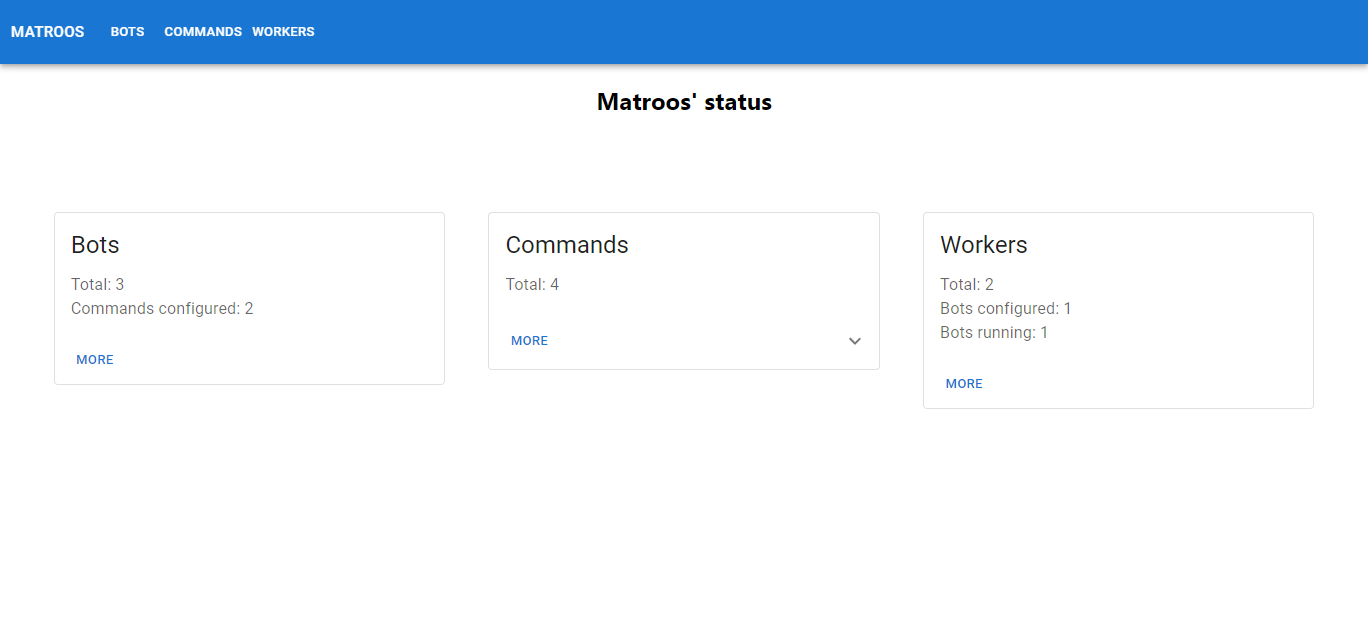
\includegraphics[width=1\textwidth]{img/front/page-home.png}
	\caption{Página principal de Matroos.}
\end{figure}

\subsubsection{Bots}

Listado de los bots disponibles, junto con modales para crear y editar bots.

\begin{figure}[H]
	\centering
	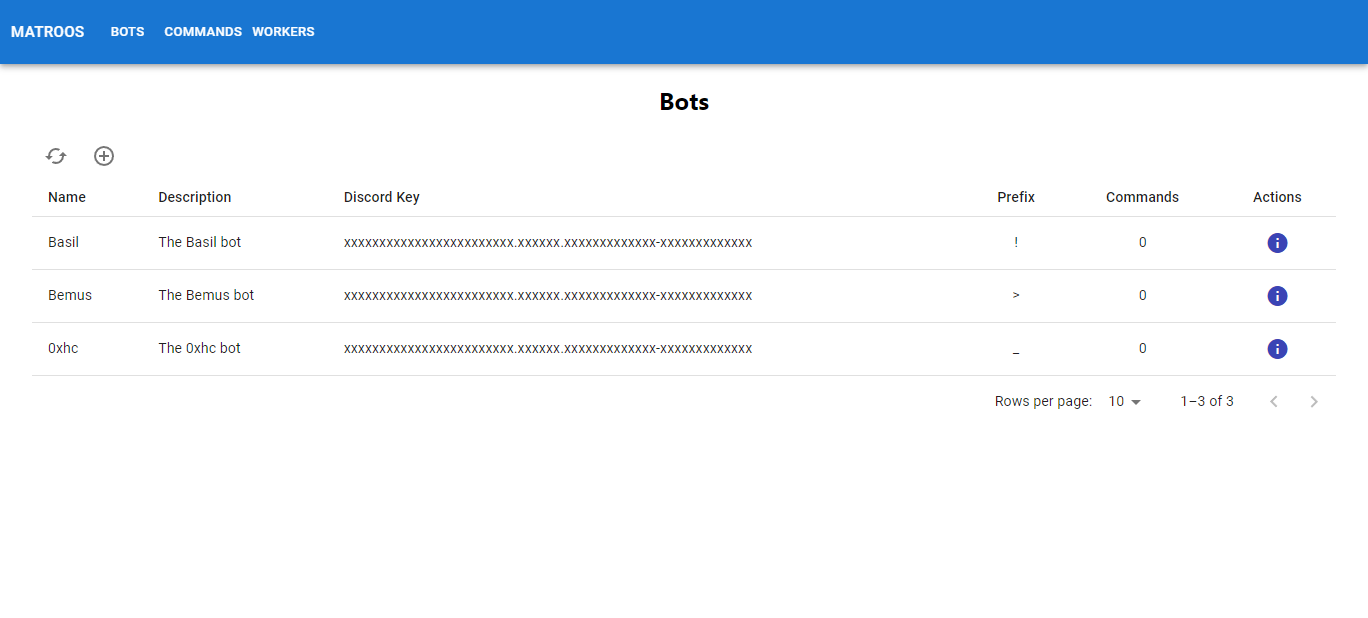
\includegraphics[width=1\textwidth]{img/front/page-bots.png}
	\caption{Página de visualización de bots.}
\end{figure}

\begin{figure}[H]
	\centering
	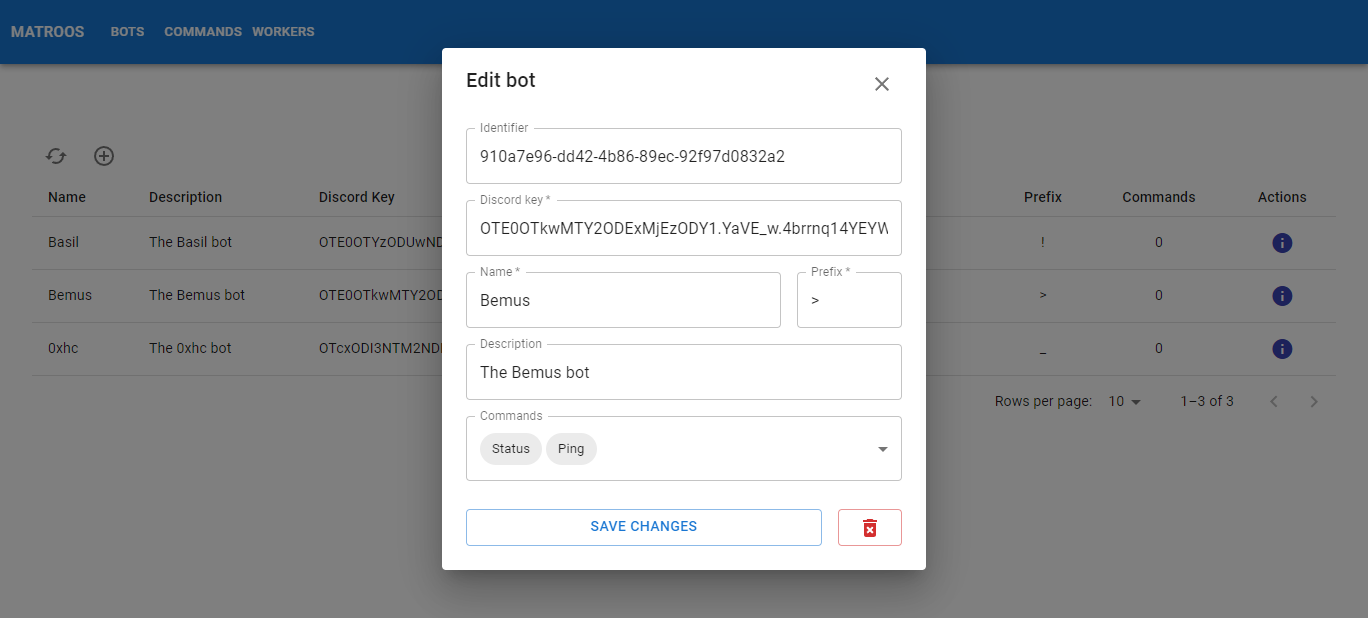
\includegraphics[width=1\textwidth]{img/front/page-bots-edit.png}
	\caption{Modal de edición de bots.}
\end{figure}

\subsubsection{Commands}

Listado de los comandos disponibles, junto con modales para crear y editar comandos.

\begin{figure}[H]
	\centering
	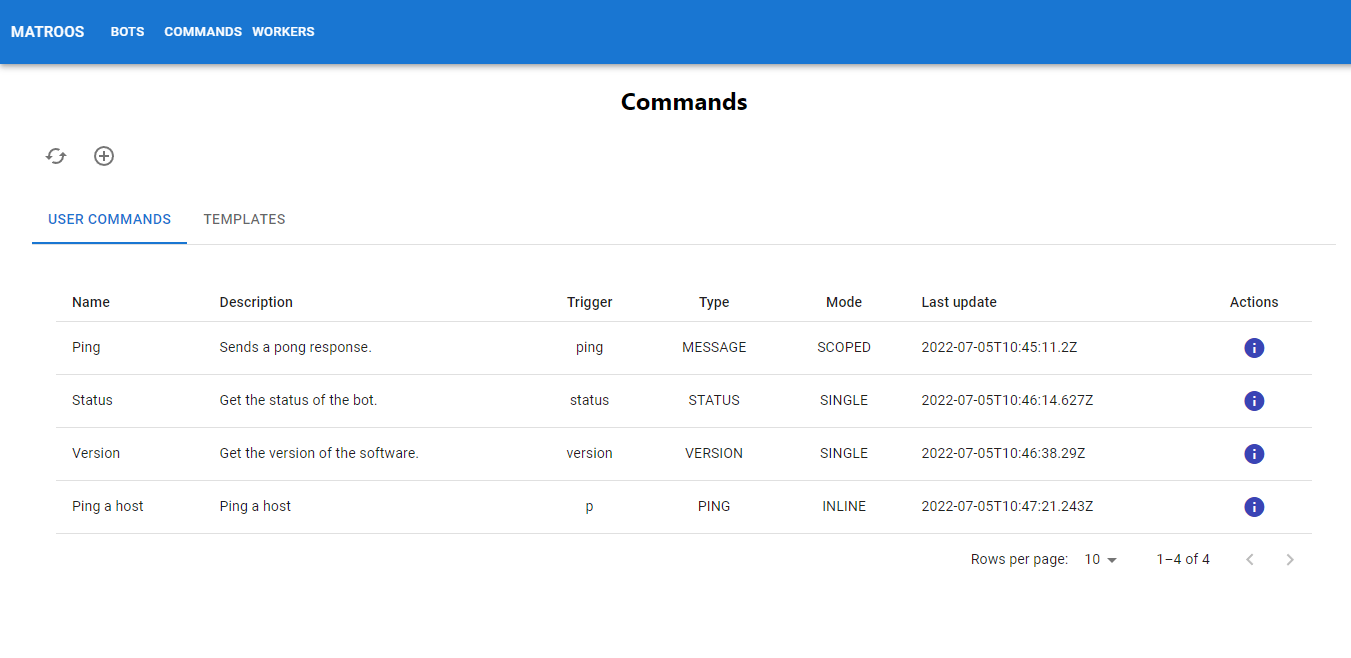
\includegraphics[width=1\textwidth]{img/front/page-commands.png}
	\caption{Página de visualización de comandos.}
\end{figure}

\begin{figure}[H]
	\centering
	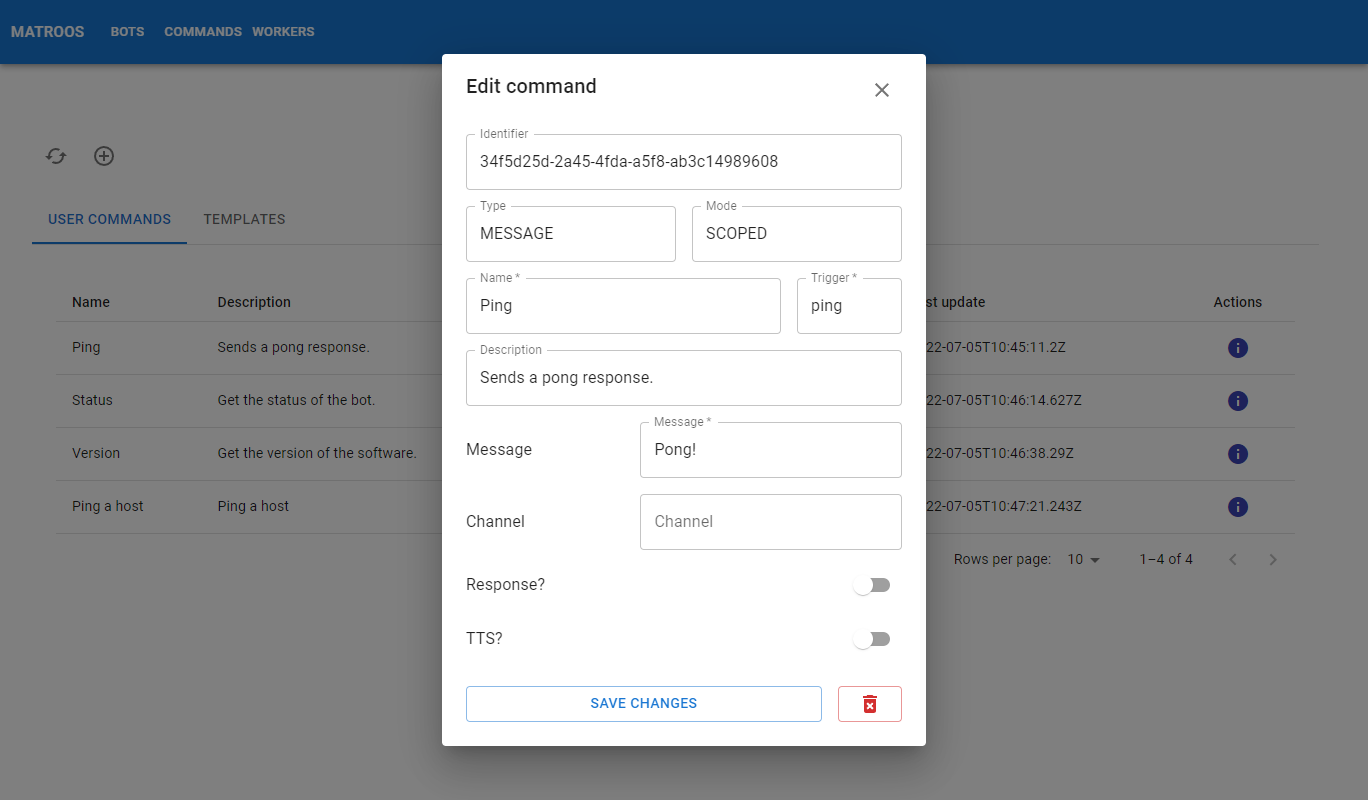
\includegraphics[width=1\textwidth]{img/front/page-commands-edit.png}
	\caption{Modal de edición de comandos.}
\end{figure}

\subsubsection{Workers}

Listado de los \textit{workers} disponibles, junto con modales para editar \textit{workers}.

\begin{figure}[H]
	\centering
	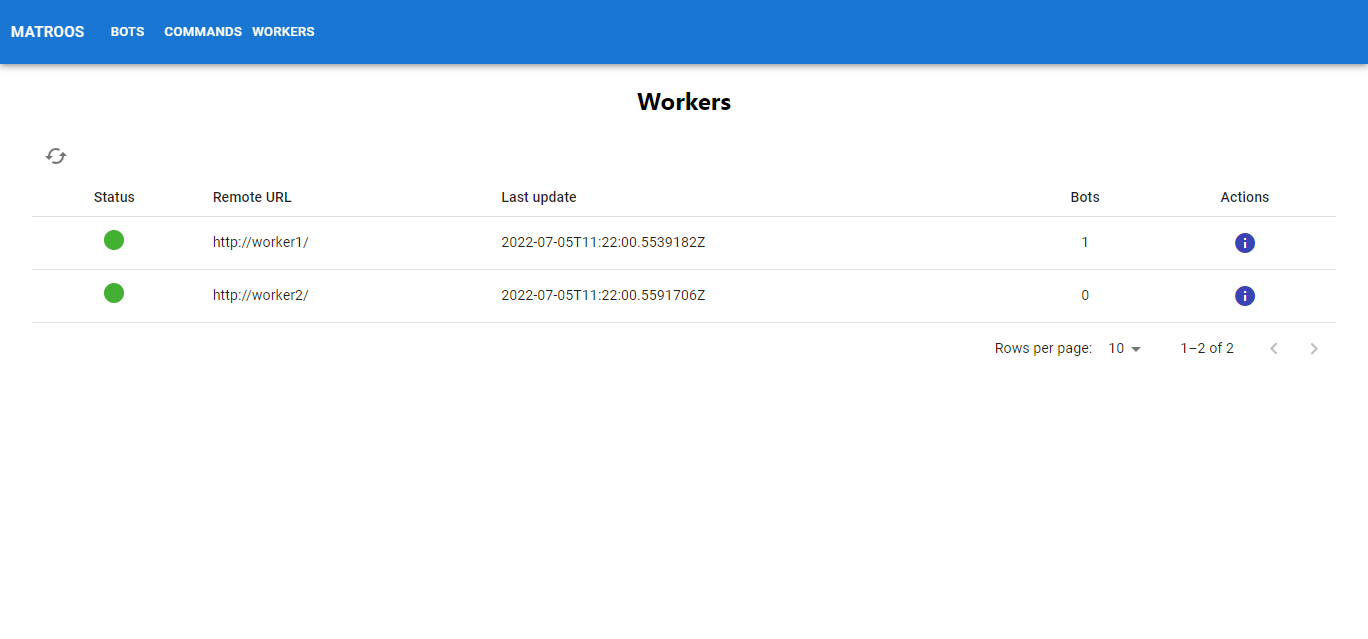
\includegraphics[width=1\textwidth]{img/front/page-workers.png}
	\caption{Página de visualización de \textit{workers}.}
\end{figure}

\begin{figure}[H]
	\centering
	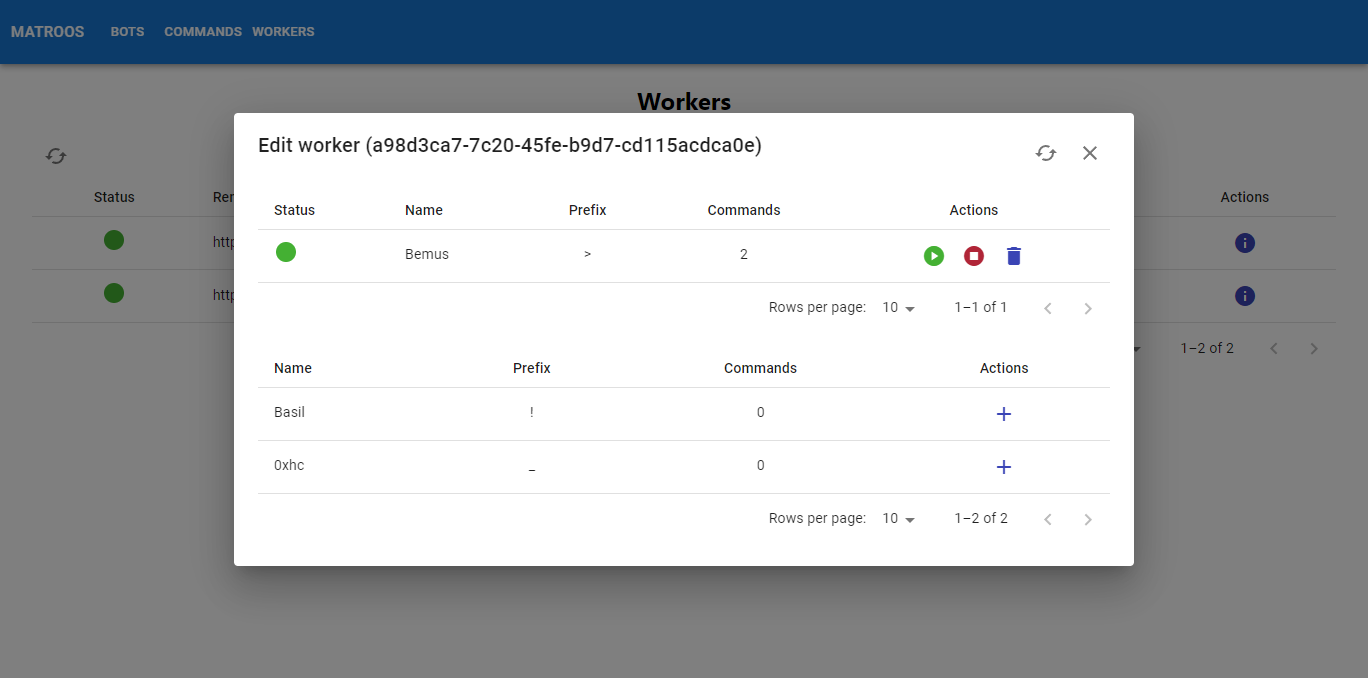
\includegraphics[width=1\textwidth]{img/front/page-workers-edit.png}
	\caption{Modal de edición de \textit{workers}.}
\end{figure}

\section{Despliegue en Docker}

Todas los microservicios que componen \textit{Matroos} son desplegables mediante contenedores \textit{Docker}. Para ello se han incluido archivos \textit{Dockerfile} para cada uno de ellos, además de archivos \textit{docker-compose.yml} para orquestar los servicios.

Además, cada vez que se hace una \textit{release} en \href{https://github.com/harvestcore/matroos}{el repositorio} de que contiene el código, se generan automáticamente nuevas imágenes de los microservicios \textit{backend} y \textit{worker}. Tras eso se suben al registro de imágenes que proporciona el propio \textit{GitHub}, \href{https://github.com/harvestcore?tab=packages&repo_name=matroos}{aquí}. Esto se ha configurado mediante un \textit{workflow} de \textit{GitHub Actions}, el cual puede encontrarse \href{https://github.com/harvestcore/matroos/blob/develop/.github/workflows/build-docker-images.yml}{aquí}.

Como se indicaba, se han incluido una serie de archivos \textit{Dockerfile} y \textit{docker-compose.yml}, son los siguientes:

\begin{lstlisting}[style=tree]
Matroos
│
├── Dockerfile.backend
├── Dockerfile.worker
│
├── docker-compose.override.yml
├── docker-compose.yml
│
└── frontend
    ├── Dockerfile
    └── docker-compose.yml
\end{lstlisting}

Para la confección de los siguientes archivos se han tenido en cuenta las mejores prácticas, intentando obtener imágenes lo más livianas posibles.

\begin{itemize}
	\item \textit{Dockerfile.backend}. Construye el microservicio \textit{backend}.
	\item \textit{Dockerfile.worker}. Construye el microservicio \textit{worker}.
	\item \textit{frontend/Dockerfile}. Construye el microservicio \textit{frontend}.
\end{itemize}

\begin{itemize}
	\item \textit{docker-compose.yml}. Orquesta tanto el microservicio \textit{backend} como el \textit{worker} haciendo uso de las imágenes subidas al registro de \textit{GitHub}. Además incluye la definición de un servicio de base de datos (\textit{MongoDB}).
	\item \textit{docker-compose.override.yml}. Igual que el anterior, pero en lugar de usar las imágenes del registro, construye las imágenes localmente.
	\item \textit{frontend/docker-compose.yml}. Orquesta el microservicio \textit{frontend}.
\end{itemize}


\section{Despliegue en producción}

Para realizar un despliegue en producción de podrían utilizar desde servidores domésticos como plataformas \textit{cloud} de gran complejidad. En el caso de \textit{Matroos}, y a modo de entorno para mostrar el funcionamiento del software se ha realizado un despliegue en un servidor \textit{cloud} dedicado, se encuentra en este \href{https://0xhc.com:9000/}{enlace}.

Como se indicaba en la sección anterior, existen distintos archivos que permiten desplegar el software mediante contenedores de \textit{Docker}, y esta plataforma es la que se ha utilizado para el despliegue en producción.

La estructura de este despliegue es la siguiente:

\begin{figure}[H]
	\centering
	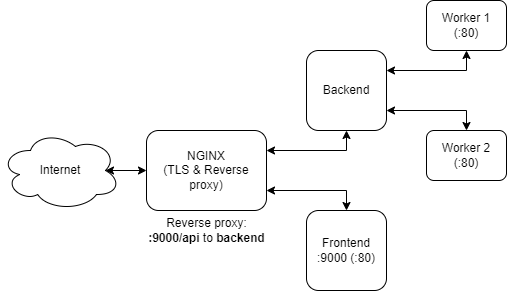
\includegraphics[width=1\textwidth]{img/production.png}
	\caption{Arquitectura del despliegue en producción.}
\end{figure}

Para conseguir esta configuración han sido necesarios algunos cambios en los archivos anteriores, además de ser necesarios algunos archivos nuevos y algunas configuraciones extra.

\subsection{Configuración de \textit{NGINX}}

El siguiente extracto muestra la configuración de un contenedor de \textit{Docker} de \textit{NGINX}.

\textbf{\textit{docker-compose.yml}}

\begin{lstlisting}[language=sh]
version: "3.3"
services:
  nginx:
    image: nginx:alpine
    container_name: nginx
    restart: always
    ports:
      - "9000:9000"   # Matroos frontend
    volumes:
      - ./nginx.conf:/etc/nginx/conf.d/default.conf
      - ./certs:/etc/nginx/certs

networks:
  default:
    external:
      name: nginx-network
\end{lstlisting}

Se puede observar que se está usando una red externa. El uso de esta permite que diferentes contenedores que se han orquestado y lanzado desde distintos archivos \textit{docker-compose.yml} compartan una misma red, y por tanto puedan comunicarse entre ellos.

\bigskip

\textbf{\textit{nginx.conf}}

\begin{lstlisting}[language=sh]
server {
    listen      9000 ssl;
    server_name 0xhc.com;

    add_header Strict-Transport-Security "max-age=31536000; includeSubDomains" always;

    error_page 497 @force_https;

    location @force_https {
        return 301 https://$host:9000$request_uri;
    }

    ssl_certificate         /etc/nginx/certs/public.crt;
    ssl_certificate_key     /etc/nginx/certs/private.key;

    location /api/ {
        auth_basic         off;
        proxy_set_header   X-Real-IP $remote_addr;
        proxy_set_header   X-Forwarded-For $proxy_add_x_forwarded_for;
        proxy_pass         http://backend/;
        proxy_http_version 1.1;
        proxy_set_header   Upgrade $http_upgrade;
        proxy_set_header   Connection "upgrade";
        add_header Strict-Transport-Security "max-age=31536000; includeSubDomains" always;
    }

    location / {
        auth_basic         off;
        proxy_set_header   X-Real-IP $remote_addr;
        proxy_set_header   X-Forwarded-For $proxy_add_x_forwarded_for;
        proxy_pass         http://matroos-front/;
        proxy_http_version 1.1;
        proxy_set_header   Upgrade $http_upgrade;
        proxy_set_header   Connection "upgrade";
        add_header Strict-Transport-Security "max-age=31536000; includeSubDomains" always;
    }
}
\end{lstlisting}

En este caso la configuración es sencilla, haciéndose un \textit{proxy} de las peticiones a los contenedores adecuados.


\subsection{Configuración de los servicios de \textit{Matroos}}

La única modificación necesaria ha sido la agregación de la red externa compartida en los archivos \textit{docker-compose.yml}, para permitir la comunicación con el servicio de \textit{NGINX}.

\begin{lstlisting}[language=sh]
networks:
  default:
    external:
      name: nginx-network
\end{lstlisting}

Una vez se ha hecho la modificación, sólo es necesario ejecutar los contenedores, quedando así el sistema completamente desplegado.

\subsection{\textit{TLS} y seguridad}

Como se indicaba en el capítulo cinco, el sistema es inseguro, ya que no ofrece ningún tipo de autenticación. Sin embargo, también se mencionaba que hay distintas maneras de agregar capas de seguridad al sistema de manera muy sencilla con software ya existente.

Sin duda una de las más sencillas es el \textit{TLS}, y en el caso de esta configuración se ha agregado haciendo uso de un certificado proporcionado por la entidad \textit{CertBot} (\textit{Let's Encrypt}) de manera gratuita.

Además, podrían agregarse otras capas de seguridad, siendo una posible la autenticación básica (o \textit{Basic Auth}). Esta también es fácilmente configurable en \textit{NGINX} y otros sistemas. En el caso de este despliegue no se ha configurado con el fin de simplificar la configuración.

	\chapter{Conclusiones y trabajos futuros}

Se pueden extraer una serie de conclusiones respecto todas las etapas de desarrollo de este proyecto, desde la definición los objetivos iniciales, hasta las etapas de investigación y creación del código del software. El objetivo principal del proyecto era simplificar el proceso de creación y uso de bots de \textit{Discord}, y el software creado cumple con creces tanto este como los objetivos secundarios.

La herramienta simplifica ampliamente la creación de bots y comandos de \textit{Discord}, además de agilizar el proceso de configuración y despliegue de los bots. Además, sirve como plataforma de desarrollo de nuevos tipos de comandos, ofreciendo las herramientas necesarias para ampliar el repertorio disponible de forma sencilla. Por otro lado, su distribución es sencilla y permite que se pueda iniciar el software, crear y configurar un bot en pocos minutos.

\section{Conclusiones}

\begin{enumerate}
	\item En este proyecto se proponía la simplificación de la creación de bots para la aplicación \textit{Discord}. Esta tarea, aunque puede parecer sencilla, una vez que se profundiza en ella no lo es. Sin embargo, proponer objetivos que pueden parecer muy exigentes y difíciles de alcanzar es una gran manera de forzar la búsqueda de la excelencia. Por tanto, con este proyecto se ha impulsado el interés por diseñar una estructura y arquitectura flexible, ambiciosa, y de gran potencial en este campo.
	
	\item Actualmente existen una cantidad de herramientas y recursos relacionados con los bots que es abrumadora, también existen para procesos como el despliegue del software. Matroos aúna todo ello en un mismo paquete, permitiendo crear y desplegar bots de una manera sencilla.

	\item \textit{Discord} es una herramienta que está creciendo mucho en muy poco tiempo. Sus usuarios requieren características concretas y complejas que la propia plataforma no ofrece. Software como el creado permite aunar de una forma sencilla muchos procesos internos, dejando disponibles a los usuarios aspectos como la ampliación del repertorio de comandos que permiten adaptar el software a cualquier situación.

	\item Crear bots desde cero implica contar con una serie de conocimientos tecnológicos de los que no todos los usuarios disponen. Herramientas como \textit{Matroos}, que facilitan esta creación y configuración, son muy valoradas y necesitadas por estos usuarios. Uno de los objetivos era reducir el tiempo de creación y despliegue de un bot al menos  un 50\%, y se ha alcanzado con creces. El desarrollo de un bot de la forma tradicional se puede demorar hasta dos horas, mientras que usando \textit{Matroos} el tiempo se reduce a no más de 10 minutos.

	\item Crear soluciones de \textit{software libre} es realmente beneficioso. La inmensa mayoría de librerías y recursos relacionados con el desarrollo de bots son de este tipo, y publicar cualquier contenido de esta manera no hace más que promover el crecimiento de las comunidades de desarrollo de software.
\end{enumerate}





\section{Trabajos futuros}

Hay algunos aspectos que podrían ser objetivo de mejora, son los siguientes:

\begin{itemize}
	\item Incrementar la cantidad de comandos predefinidos disponible. En este proyecto se han desarrollado cinco tipos de comandos disponibles para el uso de los usuarios. Si bien no es un mal comienzo ya que estos sirven como ejemplo, ampliar este repertorio es sin duda la principal rama de mejora del software.
	\item Interfaz de usuario. Aunque se ha intentado desarrollar una interfaz de usuario sencilla y fácil de utilizar, no es la más atractiva. Sin lugar a dudas es la parte principal que un usuario va a ver cuando utilice el software, por lo que su diseño y elementos visuales podrían mejorarse. Esto evitaría la pérdida de aquellos usuarios que principalmente se guían por el aspecto del software, en lugar de por las funcionalidades de este.
	\item Integración con otros sistemas y plataformas. Tanto \textit{Discord} como los frameworks de desarrollo de bots permiten la integración con redes sociales, videojuegos y otras plataformas. Sería interesante incluir utilidades internas en el software para facilitar esta conexión.
	\item \textit{Logs}. Estos son realmente importantes, ya que facilitan la trazabilidad de errores y problemas en un sistema. Aunque el software cuenta con un sistema de \textit{logging} básico, sería interesante ampliarlo para facilitar aún más la detección de errores.
\end{itemize}

	
	\appendix
	\chapter{Especificación de \textit{endpoints}}

\section{Esquemas}

\subsection{Bot}
\begin{table}[H]
    \centering
    \def\arraystretch{1.25}
    \begin{adjustbox}{max width=\textwidth}
    \begin{tabularx}{\textwidth}{|L|l|l|}
    \hline
        \textbf{\textit{Nombre}} & \textbf{\textit{Esquema}} & \textbf{\textit{Requerido}} \\ \hline
    \hline
        id & string(UUID) & Sí \\ \hline
        name & string & Sí \\ \hline
        description & string & Sí \\ \hline
        key & string & Sí \\ \hline
        prefix & string & Sí \\ \hline
        userCommands & []UserCommand & Sí \\ \hline
    \end{tabularx}
    \end{adjustbox}
\end{table}

\subsection{\textit{CommandMode}}
\begin{table}[H]
    \centering
    \def\arraystretch{1.25}
    \begin{adjustbox}{max width=\textwidth}
    \begin{tabularx}{\textwidth}{|L|l|}
    \hline
        \textbf{\textit{Propiedad}} & \textbf{\textit{Valor}} \\ \hline
    \hline
        INLINE & 0 \\ \hline
        SCOPED & 1 \\ \hline
        HEADLESS & 2 \\ \hline
        SINGLE & 3 \\ \hline
    \end{tabularx}
    \end{adjustbox}
\end{table}

\subsection{\textit{CommandSignature}}
\begin{table}[H]
    \centering
    \def\arraystretch{1.25}
    \begin{adjustbox}{max width=\textwidth}
    \begin{tabularx}{\textwidth}{|L|l|l|}
    \hline
        \textbf{\textit{Nombre}} & \textbf{\textit{Esquema}} & \textbf{\textit{Requerido}} \\ \hline
    \hline
        type & CommandType & Sí \\ \hline
        Signature & []ParameterSignature & Sí \\ \hline
        allowedModes & []CommandMode & Sí \\ \hline
    \end{tabularx}
    \end{adjustbox}
\end{table}

\subsection{\textit{CommandType}}
\begin{table}[H]
    \centering
    \def\arraystretch{1.25}
    \begin{adjustbox}{max width=\textwidth}
    \begin{tabularx}{\textwidth}{|L|l|}
    \hline
        \textbf{\textit{Propiedad}} & \textbf{\textit{Valor}} \\ \hline
    \hline
        MESSAGE & 0 \\ \hline
        PING & 1 \\ \hline
        STATUS & 2 \\ \hline
        TIMER & 3 \\ \hline
        VERSION & 4 \\ \hline
    \end{tabularx}
    \end{adjustbox}
\end{table}

\subsection{\textit{DataType}}
\begin{table}[H]
    \centering
    \def\arraystretch{1.25}
    \begin{adjustbox}{max width=\textwidth}
    \begin{tabularx}{\textwidth}{|L|l|}
    \hline
        \textbf{\textit{Propiedad}} & \textbf{\textit{Valor}} \\ \hline
    \hline
        BOOLEAN & 0 \\ \hline
        DATE & 1 \\ \hline
        DOUBLE & 2 \\ \hline
        INTEGER & 3 \\ \hline
        STRING & 4 \\ \hline
        LIST & 5 \\ \hline
    \end{tabularx}
    \end{adjustbox}
\end{table}

\subsection{\textit{ItemsResponse}}
\begin{table}[H]
    \centering
    \def\arraystretch{1.25}
    \begin{adjustbox}{max width=\textwidth}
    \begin{tabularx}{\textwidth}{|L|l|l|}
    \hline
        \textbf{\textit{Nombre}} & \textbf{\textit{Esquema}} & \textbf{\textit{Requerido}} \\ \hline
    \hline
        count & integer & Sí \\ \hline
        items & []object & Sí \\ \hline
    \end{tabularx}
    \end{adjustbox}
\end{table}

\subsection{\textit{MessageResponse}}
\begin{table}[H]
    \centering
    \def\arraystretch{1.25}
    \begin{adjustbox}{max width=\textwidth}
    \begin{tabularx}{\textwidth}{|L|l|l|}
    \hline
        \textbf{\textit{Nombre}} & \textbf{\textit{Esquema}} & \textbf{\textit{Requerido}} \\ \hline
    \hline
    	msg & string & Sí \\ \hline
    \end{tabularx}
    \end{adjustbox}
\end{table}

\subsection{\textit{ParameterSignature}}
\begin{table}[H]
    \centering
    \def\arraystretch{1.25}
    \begin{adjustbox}{max width=\textwidth}
    \begin{tabularx}{\textwidth}{|L|l|l|}
    \hline
        \textbf{\textit{Nombre}} & \textbf{\textit{Esquema}} & \textbf{\textit{Requerido}} \\ \hline
    \hline
        name & string & Sí \\ \hline
        displayName & string & Sí \\ \hline
        required & boolean & Sí \\ \hline
        type & []DataType & Sí \\ \hline
        default & object & Sí \\ \hline
    \end{tabularx}
    \end{adjustbox}
\end{table}

\subsection{\textit{SuccessResponse}}
\begin{table}[H]
    \centering
    \def\arraystretch{1.25}
    \begin{adjustbox}{max width=\textwidth}
    \begin{tabularx}{\textwidth}{|L|l|l|}
    \hline
        \textbf{\textit{Nombre}} & \textbf{\textit{Esquema}} & \textbf{\textit{Requerido}} \\ \hline
    \hline
    	success & boolean & Sí \\ \hline
    \end{tabularx}
    \end{adjustbox}
\end{table}

\subsection{\textit{UserCommand}}
\begin{table}[H]
    \centering
    \def\arraystretch{1.25}
    \begin{adjustbox}{max width=\textwidth}
    \begin{tabularx}{\textwidth}{|L|l|l|}
    \hline
        \textbf{\textit{Nombre}} & \textbf{\textit{Esquema}} & \textbf{\textit{Requerido}} \\ \hline
    \hline
        id & string(UUID) & Sí \\ \hline
        name & string & Sí \\ \hline
        description & string & Sí \\ \hline
        type & []CommandType & Sí \\ \hline
        trigger & string & Sí \\ \hline
        mode & []CommandMode & Sí \\ \hline
        parameters & object & Sí \\ \hline
    \end{tabularx}
    \end{adjustbox}
\end{table}

\subsection{\textit{Worker}}
\begin{table}[H]
    \centering
    \def\arraystretch{1.25}
    \begin{adjustbox}{max width=\textwidth}
    \begin{tabularx}{\textwidth}{|L|l|l|}
    \hline
        \textbf{\textit{Nombre}} & \textbf{\textit{Esquema}} & \textbf{\textit{Requerido}} \\ \hline
    \hline
        id & string(UUID) & Sí \\ \hline
        remoteUrl & string & Sí \\ \hline
        bots & []Bot & Sí \\ \hline
        lastUpdate & date & Sí \\ \hline
        isUp & boolean & Sí \\ \hline
    \end{tabularx}
    \end{adjustbox}
\end{table}








\section{Bots}

\subsection{\textit{GET /bots}}

\subsubsection{Parámetros}
No aplica.

\subsubsection{Respuestas}
\begin{table}[H]
    \centering
    \def\arraystretch{1.25}
    \begin{adjustbox}{max width=\textwidth}
    \begin{tabularx}{\textwidth}{|l|l|l|L|}
    \hline
        \textbf{\textit{Código}} & \textbf{\textit{Significado}} & \textbf{\textit{Descripción}} & \textbf{\textit{Esquema}} \\ \hline
    \hline
        200 & OK & Success & ItemsResponse<Bot> \\ \hline
    \end{tabularx}
    \end{adjustbox}
\end{table}




\subsection{\textit{POST /bots}}

\subsubsection{Parámetros}
\begin{table}[H]
    \centering
    \def\arraystretch{1.25}
    \begin{adjustbox}{max width=\textwidth}
    \begin{tabularx}{\textwidth}{|l|l|L|l|}
    \hline
        \textbf{\textit{Nombre}} & \textbf{\textit{En}} & \textbf{\textit{Esquema}} & \textbf{\textit{Requerido}} \\ \hline
    \hline
        - & body & Bot & Sí \\ \hline
    \end{tabularx}
    \end{adjustbox}
\end{table}

\subsubsection{Respuestas}
\begin{table}[H]
    \centering
    \def\arraystretch{1.25}
    \begin{adjustbox}{max width=\textwidth}
    \begin{tabularx}{\textwidth}{|l|l|l|L|}
    \hline
        \textbf{\textit{Código}} & \textbf{\textit{Significado}} & \textbf{\textit{Descripción}} & \textbf{\textit{Esquema}} \\ \hline
    \hline
        200 & OK & Success & ItemsResponse<Bot> \\ \hline
        400 & Bad Request & Failure & - \\ \hline
    \end{tabularx}
    \end{adjustbox}
\end{table}





\subsection{\textit{PUT /bots}}

\subsubsection{Parámetros}
\begin{table}[H]
    \centering
    \def\arraystretch{1.25}
    \begin{adjustbox}{max width=\textwidth}
    \begin{tabularx}{\textwidth}{|l|l|L|l|}
    \hline
        \textbf{\textit{Nombre}} & \textbf{\textit{En}} & \textbf{\textit{Esquema}} & \textbf{\textit{Requerido}} \\ \hline
    \hline
        - & body & Bot & Sí \\ \hline
    \end{tabularx}
    \end{adjustbox}
\end{table}

\subsubsection{Respuestas}
\begin{table}[H]
    \centering
    \def\arraystretch{1.25}
    \begin{adjustbox}{max width=\textwidth}
    \begin{tabularx}{\textwidth}{|l|l|l|L|}
    \hline
        \textbf{\textit{Código}} & \textbf{\textit{Significado}} & \textbf{\textit{Descripción}} & \textbf{\textit{Esquema}} \\ \hline
    \hline
        200 & OK & Success & SuccessResponse \\ \hline
        400 & Bad Request & Failure & MessageResponse \\ \hline
    \end{tabularx}
    \end{adjustbox}
\end{table}





\subsection{\textit{GET /bots/\{botId\}}}
\subsubsection{Parámetros}
\begin{table}[H]
    \centering
    \def\arraystretch{1.25}
    \begin{adjustbox}{max width=\textwidth}
    \begin{tabularx}{\textwidth}{|l|l|L|l|}
    \hline
        \textbf{\textit{Nombre}} & \textbf{\textit{En}} & \textbf{\textit{Esquema}} & \textbf{\textit{Requerido}} \\ \hline
    \hline
        botId & query & string & Sí \\ \hline
    \end{tabularx}
    \end{adjustbox}
\end{table}

\subsubsection{Respuestas}
\begin{table}[H]
    \centering
    \def\arraystretch{1.25}
    \begin{adjustbox}{max width=\textwidth}
    \begin{tabularx}{\textwidth}{|l|l|l|L|}
    \hline
        \textbf{\textit{Código}} & \textbf{\textit{Significado}} & \textbf{\textit{Descripción}} & \textbf{\textit{Esquema}} \\ \hline
    \hline
        200 & OK & Success & Bot \\ \hline
        404 & Not Found & Failure & - \\ \hline
    \end{tabularx}
    \end{adjustbox}
\end{table}





\subsection{\textit{DELETE /bots/\{botId\}}}
\subsubsection{Parámetros}
\begin{table}[H]
    \centering
    \def\arraystretch{1.25}
    \begin{adjustbox}{max width=\textwidth}
    \begin{tabularx}{\textwidth}{|l|l|L|l|}
    \hline
        \textbf{\textit{Nombre}} & \textbf{\textit{En}} & \textbf{\textit{Esquema}} & \textbf{\textit{Requerido}} \\ \hline
    \hline
        botId & query & string & Sí \\ \hline
    \end{tabularx}
    \end{adjustbox}
\end{table}

\subsubsection{Respuestas}
\begin{table}[H]
    \centering
    \def\arraystretch{1.25}
    \begin{adjustbox}{max width=\textwidth}
    \begin{tabularx}{\textwidth}{|l|l|l|L|}
    \hline
        \textbf{\textit{Código}} & \textbf{\textit{Significado}} & \textbf{\textit{Descripción}} & \textbf{\textit{Esquema}} \\ \hline
    \hline
        200 & OK & Success & SuccessResponse \\ \hline
        400 & Bad Request & Failure & MessageResponse \\ \hline
    \end{tabularx}
    \end{adjustbox}
\end{table}





\section{\textit{Commands}}

\subsection{\textit{GET /commands/signatures}}

\subsubsection{Parámetros}
No aplica.

\subsubsection{Respuestas}
\begin{table}[H]
    \centering
    \def\arraystretch{1.25}
    \begin{adjustbox}{max width=\textwidth}
    \begin{tabularx}{\textwidth}{|l|l|l|L|}
    \hline
        \textbf{\textit{Código}} & \textbf{\textit{Significado}} & \textbf{\textit{Descripción}} & \textbf{\textit{Esquema}} \\ \hline
    \hline
        200 & OK & Success & ItemsResponse<CommandSignature> \\ \hline
    \end{tabularx}
    \end{adjustbox}
\end{table}




\subsection{\textit{GET /commands}}

\subsubsection{Parámetros}
No aplica.

\subsubsection{Respuestas}
\begin{table}[H]
    \centering
    \def\arraystretch{1.25}
    \begin{adjustbox}{max width=\textwidth}
    \begin{tabularx}{\textwidth}{|l|l|l|L|}
    \hline
        \textbf{\textit{Código}} & \textbf{\textit{Significado}} & \textbf{\textit{Descripción}} & \textbf{\textit{Esquema}} \\ \hline
    \hline
        200 & OK & Success & ItemsResponse<UserCommand> \\ \hline
    \end{tabularx}
    \end{adjustbox}
\end{table}





\subsection{\textit{POST /commands}}

\subsubsection{Parámetros}
\begin{table}[H]
    \centering
    \def\arraystretch{1.25}
    \begin{adjustbox}{max width=\textwidth}
    \begin{tabularx}{\textwidth}{|l|l|L|l|}
    \hline
        \textbf{\textit{Nombre}} & \textbf{\textit{En}} & \textbf{\textit{Esquema}} & \textbf{\textit{Requerido}} \\ \hline
    \hline
        - & body & UserCommand & Sí \\ \hline
    \end{tabularx}
    \end{adjustbox}
\end{table}

\subsubsection{Respuestas}
\begin{table}[H]
    \centering
    \def\arraystretch{1.25}
    \begin{adjustbox}{max width=\textwidth}
    \begin{tabularx}{\textwidth}{|l|l|l|L|}
    \hline
        \textbf{\textit{Código}} & \textbf{\textit{Significado}} & \textbf{\textit{Descripción}} & \textbf{\textit{Esquema}} \\ \hline
    \hline
        200 & OK & Success & SuccessResponse \\ \hline
        400 & Bad Request & Failure & MessageResponse \\ \hline
    \end{tabularx}
    \end{adjustbox}
\end{table}






\subsection{\textit{PUT /commands}}

\subsubsection{Parámetros}
\begin{table}[H]
    \centering
    \def\arraystretch{1.25}
    \begin{adjustbox}{max width=\textwidth}
    \begin{tabularx}{\textwidth}{|l|l|L|l|}
    \hline
        \textbf{\textit{Nombre}} & \textbf{\textit{En}} & \textbf{\textit{Esquema}} & \textbf{\textit{Requerido}} \\ \hline
    \hline
        - & body & UserCommand & Sí \\ \hline
    \end{tabularx}
    \end{adjustbox}
\end{table}

\subsubsection{Respuestas}
\begin{table}[H]
    \centering
    \def\arraystretch{1.25}
    \begin{adjustbox}{max width=\textwidth}
    \begin{tabularx}{\textwidth}{|l|l|l|L|}
    \hline
        \textbf{\textit{Código}} & \textbf{\textit{Significado}} & \textbf{\textit{Descripción}} & \textbf{\textit{Esquema}} \\ \hline
    \hline
        200 & OK & Success & SuccessResponse \\ \hline
        400 & Bad Request & Failure & MessageResponse \\ \hline
    \end{tabularx}
    \end{adjustbox}
\end{table}









\subsection{\textit{GET /commands/\{commandId\}}}
\subsubsection{Parámetros}
\begin{table}[H]
    \centering
    \def\arraystretch{1.25}
    \begin{adjustbox}{max width=\textwidth}
    \begin{tabularx}{\textwidth}{|l|l|L|l|}
    \hline
        \textbf{\textit{Nombre}} & \textbf{\textit{En}} & \textbf{\textit{Esquema}} & \textbf{\textit{Requerido}} \\ \hline
    \hline
        commandId & query & string(UUID) & Sí \\ \hline
    \end{tabularx}
    \end{adjustbox}
\end{table}

\subsubsection{Respuestas}
\begin{table}[H]
    \centering
    \def\arraystretch{1.25}
    \begin{adjustbox}{max width=\textwidth}
    \begin{tabularx}{\textwidth}{|l|l|l|L|}
    \hline
        \textbf{\textit{Código}} & \textbf{\textit{Significado}} & \textbf{\textit{Descripción}} & \textbf{\textit{Esquema}} \\ \hline
    \hline
        200 & OK & Success & UserCommand \\ \hline
        404 & Not Found & Failure & - \\ \hline
    \end{tabularx}
    \end{adjustbox}
\end{table}






\subsection{\textit{DELETE /commands/\{commandId\}}}
\subsubsection{Parámetros}
\begin{table}[H]
    \centering
    \def\arraystretch{1.25}
    \begin{adjustbox}{max width=\textwidth}
    \begin{tabularx}{\textwidth}{|l|l|L|l|}
    \hline
        \textbf{\textit{Nombre}} & \textbf{\textit{En}} & \textbf{\textit{Esquema}} & \textbf{\textit{Requerido}} \\ \hline
    \hline
        commandId & query & string(UUID) & Sí \\ \hline
    \end{tabularx}
    \end{adjustbox}
\end{table}

\subsubsection{Respuestas}
\begin{table}[H]
    \centering
    \def\arraystretch{1.25}
    \begin{adjustbox}{max width=\textwidth}
    \begin{tabularx}{\textwidth}{|l|l|l|L|}
    \hline
        \textbf{\textit{Código}} & \textbf{\textit{Significado}} & \textbf{\textit{Descripción}} & \textbf{\textit{Esquema}} \\ \hline
    \hline
        200 & OK & Success & SuccessResponse \\ \hline
        400 & Bad Request & Failure & MessageResponse \\ \hline
    \end{tabularx}
    \end{adjustbox}
\end{table}








\section{\textit{Workers}}




\subsection{\textit{GET /workers}}

\subsubsection{Parámetros}
No aplica.

\subsubsection{Respuestas}
\begin{table}[H]
    \centering
    \def\arraystretch{1.25}
    \begin{adjustbox}{max width=\textwidth}
    \begin{tabularx}{\textwidth}{|l|l|l|L|}
    \hline
        \textbf{\textit{Código}} & \textbf{\textit{Significado}} & \textbf{\textit{Descripción}} & \textbf{\textit{Esquema}} \\ \hline
    \hline
        200 & OK & Success & ItemsResponse<Worker> \\ \hline
    \end{tabularx}
    \end{adjustbox}
\end{table}




\subsection{\textit{GET /workers/\{workerId\}/start/\{botId\}}}
\subsubsection{Parámetros}
\begin{table}[H]
    \centering
    \def\arraystretch{1.25}
    \begin{adjustbox}{max width=\textwidth}
    \begin{tabularx}{\textwidth}{|l|l|L|l|}
    \hline
        \textbf{\textit{Nombre}} & \textbf{\textit{En}} & \textbf{\textit{Esquema}} & \textbf{\textit{Requerido}} \\ \hline
    \hline
        workerId & query & string(UUID) & Sí \\ \hline
        botId & query & string(UUID) & Sí \\ \hline
    \end{tabularx}
    \end{adjustbox}
\end{table}

\subsubsection{Respuestas}
\begin{table}[H]
    \centering
    \def\arraystretch{1.25}
    \begin{adjustbox}{max width=\textwidth}
    \begin{tabularx}{\textwidth}{|l|l|l|L|}
    \hline
        \textbf{\textit{Código}} & \textbf{\textit{Significado}} & \textbf{\textit{Descripción}} & \textbf{\textit{Esquema}} \\ \hline
    \hline
        200 & OK & Success & SuccessResponse \\ \hline
        400 & Bad Request & Failure & MessageResponse \\ \hline
    \end{tabularx}
    \end{adjustbox}
\end{table}




\subsection{\textit{GET /workers/\{workerId\}/stop/\{botId\}}}
\subsubsection{Parámetros}
\begin{table}[H]
    \centering
    \def\arraystretch{1.25}
    \begin{adjustbox}{max width=\textwidth}
    \begin{tabularx}{\textwidth}{|l|l|L|l|}
    \hline
        \textbf{\textit{Nombre}} & \textbf{\textit{En}} & \textbf{\textit{Esquema}} & \textbf{\textit{Requerido}} \\ \hline
    \hline
        workerId & query & string(UUID) & Sí \\ \hline
        botId & query & string(UUID) & Sí \\ \hline
    \end{tabularx}
    \end{adjustbox}
\end{table}

\subsubsection{Respuestas}
\begin{table}[H]
    \centering
    \def\arraystretch{1.25}
    \begin{adjustbox}{max width=\textwidth}
    \begin{tabularx}{\textwidth}{|l|l|l|L|}
    \hline
        \textbf{\textit{Código}} & \textbf{\textit{Significado}} & \textbf{\textit{Descripción}} & \textbf{\textit{Esquema}} \\ \hline
    \hline
        200 & OK & Success & SuccessResponse \\ \hline
        400 & Bad Request & Failure & MessageResponse \\ \hline
    \end{tabularx}
    \end{adjustbox}
\end{table}







\subsection{\textit{GET /workers/\{workerId\}}}
\subsubsection{Parámetros}
\begin{table}[H]
    \centering
    \def\arraystretch{1.25}
    \begin{adjustbox}{max width=\textwidth}
    \begin{tabularx}{\textwidth}{|l|l|L|l|}
    \hline
        \textbf{\textit{Nombre}} & \textbf{\textit{En}} & \textbf{\textit{Esquema}} & \textbf{\textit{Requerido}} \\ \hline
    \hline
        workerId & query & string(UUID) & Sí \\ \hline
    \end{tabularx}
    \end{adjustbox}
\end{table}

\subsubsection{Respuestas}
\begin{table}[H]
    \centering
    \def\arraystretch{1.25}
    \begin{adjustbox}{max width=\textwidth}
    \begin{tabularx}{\textwidth}{|l|l|l|L|}
    \hline
        \textbf{\textit{Código}} & \textbf{\textit{Significado}} & \textbf{\textit{Descripción}} & \textbf{\textit{Esquema}} \\ \hline
    \hline
        200 & OK & Success & Worker \\ \hline
        404 & Not Found & Failure & - \\ \hline
    \end{tabularx}
    \end{adjustbox}
\end{table}






\subsection{\textit{POST /workers/\{workerId\}}}
\subsubsection{Parámetros}
\begin{table}[H]
    \centering
    \def\arraystretch{1.25}
    \begin{adjustbox}{max width=\textwidth}
    \begin{tabularx}{\textwidth}{|l|l|L|l|}
    \hline
        \textbf{\textit{Nombre}} & \textbf{\textit{En}} & \textbf{\textit{Esquema}} & \textbf{\textit{Requerido}} \\ \hline
    \hline
        workerId & query & string(UUID) & Sí \\ \hline
        - & body & []string(UUID) & Sí \\ \hline
    \end{tabularx}
    \end{adjustbox}
\end{table}

\subsubsection{Respuestas}
\begin{table}[H]
    \centering
    \def\arraystretch{1.25}
    \begin{adjustbox}{max width=\textwidth}
    \begin{tabularx}{\textwidth}{|l|l|l|L|}
    \hline
        \textbf{\textit{Código}} & \textbf{\textit{Significado}} & \textbf{\textit{Descripción}} & \textbf{\textit{Esquema}} \\ \hline
    \hline
        200 & OK & Success & SuccessResponse \\ \hline
        400 & Bad Request & Failure & MessageResponse \\ \hline
    \end{tabularx}
    \end{adjustbox}
\end{table}






\subsection{\textit{DELETE /workers/\{workerId\}}}
\subsubsection{Parámetros}
\begin{table}[H]
    \centering
    \def\arraystretch{1.25}
    \begin{adjustbox}{max width=\textwidth}
    \begin{tabularx}{\textwidth}{|l|l|L|l|}
    \hline
        \textbf{\textit{Nombre}} & \textbf{\textit{En}} & \textbf{\textit{Esquema}} & \textbf{\textit{Requerido}} \\ \hline
    \hline
        workerId & query & string(UUID) & Sí \\ \hline
        - & body & []string(UUID) & Sí \\ \hline
    \end{tabularx}
    \end{adjustbox}
\end{table}

\subsubsection{Respuestas}
\begin{table}[H]
    \centering
    \def\arraystretch{1.25}
    \begin{adjustbox}{max width=\textwidth}
    \begin{tabularx}{\textwidth}{|l|l|l|L|}
    \hline
        \textbf{\textit{Código}} & \textbf{\textit{Significado}} & \textbf{\textit{Descripción}} & \textbf{\textit{Esquema}} \\ \hline
    \hline
        200 & OK & Success & SuccessResponse \\ \hline
        400 & Bad Request & Failure & MessageResponse \\ \hline
    \end{tabularx}
    \end{adjustbox}
\end{table}
	\chapter{Variables de entorno}

\textbf{Matroos} hace uso de algunas variables de entorno para funcionar correctamente que deben ser configuradas. Son las siguientes:

\begin{itemize}
	\item \textsf{MongoDBConnectionString}. \textit{String} de conexión al servidor de \textit{MongoDB}. \\ E.g.: \textsf{mongodb://mongodb:27017/matroos}
	\item \textsf{MongoDBDatabaseName}. Nombre de la base de datos. \\ E.g.: \textsf{matroos}
	\item \textsf{TestMongoDBConnectionString}. \textit{String} de conexión al servidor de \textit{MongoDB} para ejecutar las pruebas unitarias. \\ E.g.: \textsf{mongodb://mongodb:27017/matroos-test}
	\item \textsf{TestMongoDBDatabaseName}. Nombre de la base de datos para ejecutar las pruebas unitarias. \\ E.g.: \textsf{matroos-test}
	\item \textsf{Workers}. URLs de los \textit{workers} desplegados separadas por ''\textsf{;}``. \\ E.g.: \textsf{http://worker1/;http://worker2/}
\end{itemize}

	\chapter{Instalación del sistema}

Una vez se ha clonado \href{https://github.com/harvestcore/matroos}{el repositorio} se puede instalar el software siguiendo los pasos que se describen a continuación.

\section{\textit{Backend} y \textit{workers}}


Para ejecutar estos servicios se recomienda el uso de \textit{Visual Studio}, ya que facilita mucho este proceso. Aún así, se puede ejecutar mediante línea de comandos:

\begin{lstlisting}
cd matroos

// Compilar Backend.
cd backend
dotnet restore
dotnet build --no-restore -c Release
dotnet publish -c Release -o ./app --no-restore

// Compilar Worker.
cd worker
dotnet restore
dotnet build --no-restore -c Release
dotnet publish -c Release -o ./app --no-restore


// Ejecutar backend.
cd backend/app
dotnet Matroos.Backend.dll


// Ejecutar worker.
cd worker/app
dotnet Matroos.Worker.dll
\end{lstlisting}

En cambio, para ejecutar de una manera mucho más sencilla los servicios, se puede usar \textit{Docker}.

\begin{lstlisting}[language=sh]
cd matroos

// Construir imagenes.
docker-compose build

// Ejecutar contenedores.
docker-compose up
\end{lstlisting}

Además, previa ejecución de los servicios, se deben revisar las variables de entorno.




\section{Frontend}

Ejecución del \textit{frontend} instalando y construyendo el servicio de manera local:

\begin{lstlisting}[language=sh]
cd matroos/frontend

// Instalación de dependencias.
npm install

// Ejecución de un entorno de pruebas.
npm run start

// Construcción de una versión de producción.
npm run build
\end{lstlisting}

En el caso de utilizar una \textit{build} de producción se recomienda utilizar un servidor web como \textit{NGINX}, aunque puede usarse cualquier otro.

Por otro lado se puede ejecutar el \textit{frontend} haciendo uso de \textit{Docker}, para ello es necesario ejecutar:

\begin{lstlisting}[language=sh]
cd matroos/frontend

// Construir imagen.
docker-compose build

// Ejecutar contenedor.
docker-compose up
\end{lstlisting}

De cualquier modo, previa ejecución del \textit{frontend} debe configurarse la variable \textit{BACKEND\_URL}, la cual se encuentra en el archivo \textit{frontend/api/fetch.ts}. En un ambiente local puede definirse la variable de entorno con ese mismo nombre, en el caso de una \textit{build} de producción o en el uso de \textit{Docker} debe asignarse esa variable manualmente.

	
	\newpage
	\bibliography{biblio}
	\bibliographystyle{plain}
	
\end{document}

